\documentclass[utf8]{gradu3}
% Jos työ on kandidaatintutkielma eikä pro gradu, käytä ylläolevan asemesta
%\documentclass[utf8,bachelor]{gradu3}
% Jos kirjoitat englanniksi, käytä ylläolevan asemesta
%\documentclass[utf8,english]{gradu3}
% tai
%\documentclass[utf8,bachelor,english]{gradu3}

\usepackage{graphicx} % kuvien mukaan ottamista varten

\usepackage{amsmath} % hyödyllinen jos tekstisi sisältää matikkaa,
                     % ei pakollinen

\usepackage{booktabs} % hyvä kauniiden taulukoiden tekemiseen

\usepackage[authordate,backend=biber,noibid]{biblatex-chicago} % biber / chicago-tyylin käyttö

\usepackage{graphicx} % kuvien lisääminen

% HUOM! Tämän tulee olla viimeinen \usepackage koko dokumentissa!
\usepackage[bookmarksopen,bookmarksnumbered,linktocpage]{hyperref}

\addbibresource{gradu_EK.bib} % Lähdetietokannan tiedostonimi

\begin{document}

\title{Vertaileva tutkimus koneoppimisen hyödyntämisestä videopelien reitinhaussa}
\translatedtitle{Comparative study of utilizing machine learning in video games' pathfinding}
\studyline{Tietotekniikka}
\tiivistelma{%
Reitinhaku on yksi suurimmista ongelmista tekoälyn tutkimuksessa. Viime vuosikymmenten aikana sekä robotiikan että videopelien reitinhakuongelmat ovat tuottaneet erilaisia ratkaisuja kuten A*-algoritmi ja sen variaatiot. Videopeleissä etenkin A*-algoritmia on pidetty luotettavana ratkaisuna sen optimaalisuuden takia. Dynaamiset pelialueet ja moniagenttireitinhaku ovat kuitenkin tuoneet haasteita, joihin A*-algoritmi ei ole pystynyt yksin vastaamaan. Tässä tutkimuksessa hyödynnetään Unity-pelinkehitysalustalle luotua ML-agents-pakettia koneoppimisagentin luomiseen ja testataan sen soveltuvuutta reitinhakutehtäviin. Koneoppimisagentit käyttävät syvää vahvistusoppimista ja siihen perustuvaa Soft Actor-Critic -algoritmia. Lopuksi tarkoituksena on vertailla perinteisen A*-algoritmin tuloksia koneoppimisagentin tuloksiin.
}
\abstract{%
Pathfinding or path planning is one of the major problems in AI research. During the last decades pathfinding in both robotics and video games has produced different solutions like A*-algorithm and its variations. In video games especially A*-algorithm has been the reliable solution because of its optimality. Dynamic video game environments and multi-agent pathfinding have brought challenges where A*-algorithm alone has proven to be insufficient. In this thesis Unity platform and its ML-agents-package will be used to create machine learning agent for executing pathfinding tasks. Machine learning agent uses deep reinforcement learning and Soft Actor-Critic -algorithm. Lastly A*-based solutions and machine learning agents will be compared against each other.
}

\author{Emil Keränen}
\contactinformation{\texttt{keranen.emil@gmail.com}}
% jos useita tekijöitä, anna useampi \author-komento
\supervisor{Tommi Kärkkäinen}
% jos useita ohjaajia, anna useampi \supervisor-komento
\avainsanat{koneoppiminen, videopeli, reitinhaku, syvä vahvistusoppiminen}
\keywords{machine learning, video game, pathfinding, deep reinforcement learning, Soft Actor-Critic, Machine Learning Agents, Unity}

\maketitle

\bigskip

\mainmatter

\chapter{Johdanto}

Reitinhaku on robotiikan ja videopelien tekoälyn yksi suurimmista ongelmista, jota on tutkittu jo vuosikymmeniä \parencite{abd2015comprehensive,cui2011based}. Reitinhaulla tarkoitetaan kahden pisteen tai solmun välisen reitin selvittämistä alueella, jossa on vapaita solmuja ja estesolmuja. Useimmissa tapauksissa halutaan etsiä nopein ja tehokkain reitti, mutta ongelman haastavuuden vuoksi voidaan tyytyä myös epäoptimaalisiin ratkaisuihin \parencite{rahmani2022towards}. Reitinhakuongelma on ajan mittaan muuttunut lyhimmän reitin löytämisestä myös reitin selvittämiseen muuttuvassa eli dynaamisessa alueessa. Erityisesti robottien suorittamaa dynaamisen alueen reitinhakua on tutkittu viime vuosina ja siten uudet vaatimukset, kuten turvallisuus ja tarkkuus, ovat nousseet prioriteeteissa \parencite{karur2021survey}.

Usein perinteinen reitinhakuongelma pystytään ratkaisemaan A*-algoritmilla, jota käytetään etenkin videopeleissä, mutta myös robotiikassa \parencite{abd2015comprehensive,botea2013pathfinding,cui2011based}. A*-algoritmi löytää optimaalisen reitin heuristiikkafunktion ansiosta. Heuristiikkafunktion avulla algoritmin ei tarvitse tutkia selvästi huonompia vaihtoehtoja, jolloin reitinhausta saadaan kevyempää.

Videopeleissä reitinhaku ilmenee usein erillisten tekoälyagenttien toimintana. Näitä kutsutaan myös ei-pelaaja-hahmoiksi (engl. non-player-character, NPC) \parencite{cui2011based}. Videopelien reitinhaussa suorituskyky nousee suurimmaksi ongelmaksi. Tietokoneen suorituskyky osoittautuu rajalliseksi vaativien grafiikka- ja fysiikkalaskelmien vuoksi. Joissain peleissä, kuten reaaliaikaisissa strategiapeleissä (engl. Real-Time Strategy, RTS), pelaajan ohjaamia liikkuvia hahmoja voi olla samanaikaisesti jopa satoja, joten esimerkiksi pelkän A*-algoritmin soveltaminen jokaiselle agentille osoittautuu äärimmäisen haastavaksi laskennallisesti. Siksi vuosien mittaan on kehitetty ratkaisuksi erilaisia pelialueen esitystavan muokkauksia, reitinhakualgoritmien variaatioita ja lopulta jopa koneoppimisratkaisuja.

Koneoppimista ja sen menetelmiä on myös tutkittu viime vuosina hyvin paljon eri sovellusten parissa \parencite{jordan2015machine}. Koneoppimisen avulla pystytään hyödyntämään aiempaa kokemusta uusissa tilanteissa. Etenkin neuroverkkoja ja syväoppimista on pystytty hyödyntämään monissa erilaisissa ongelmissa luokittelusta robotiikkaan.

Tässä tutkimuksessa on tarkoitus soveltaa Unity-pelinkehitysalustan valmista Machine Learning Agents -pakettia (ML-agents) reitinhakuagenttien luomiseen. ML-agents käyttää Py\-Torch-kirjastoa neuroverkkomallin luomiseen. ML-agents-paketin avulla agentteja voidaan opettaa reitinhakuun käyttäen syvää vahvistusoppimista ja siihen perustuvaa Soft Actor Critic -algoritmia. Tarkoitus on pyrkiä vastaamaan seuraaviin tutkimuskysymyksiin

\begin{enumerate}
\item Oppiiko koneoppimisagentti suorittamaan reitinhakutehtäviä?
\item Miten koneoppimisagentin suorittama reitinhaku vertautuu A*-algoritmiin nopeuden ja tarkkuuden osalta?
\item Löytyykö reitinhakutehtävä, jota A*-algoritmi ei pysty ratkaisemaan, mutta koneoppimisagentti pystyy?
\end{enumerate}

Luvussa \ref{reitinhakupeleis} kerrotaan yleisesti reitinhakuongelmasta videopeleissä pelialueiden esitystavan ja käytettyjen reitinhakualgoritmien muodossa. Luvussa \ref{koneoppiminen} käsitellään yleisesti koneoppimista, sen eri paradigmoja ja syväoppimista. Luvussa \ref{unity} esitellään pelinkehitysalusta Unity, sen rakenne ja tässä tutkimuksessa käytetyt paketit. Luvussa \ref{empiirinen} käydään läpi tutkimuksen empiirinen osuus menetelmien ja tutkimusasetelman kannalta. Luvussa \ref{tulokset} esitellään ja analysoidaan empiirisessä osuudessa saadut tulokset. Lopuksi luvussa \ref{yhteenveto} käydään läpi tutkimuksen yhteenveto lyhyesti.

\chapter{Reitinhaku videopeleissä}
\label{reitinhakupeleis}

Reitinhaulla tarkoitetaan yksinkertaisimmillaan reitin tai polun selvittämistä kahden pisteen välillä pelialueella. Se on yksi videopelien tekoälyn ja myös robotiikan tunnetuimmista ja haastavimmista ongelmista, jota on tutkittu jo muutaman vuosikymmenen ajan \parencite{abd2015comprehensive,cui2011based}. Reitinhakua esiintyy monissa eri peligenreissä, kuten roolipeleissä ja reaaliaikaisissa strategiapeleissä, joissa ei-pelaaja-hahmot liikkuvat ennaltamäärättyyn tai pelaajan määräämään sijaintiin väistellen samalla vastaantulevia esteitä. Reitinhaun ja yleisesti tekoälyn on oltava realistista, jotta pelaaja pystyy syventymään videopelin maailmaan eikä pelaajan kokema immersio esty.

\section{Pelialueen esitystavat}

Pelialue esitetään reitinhakua varten aina graafina, joka koostuu solmuista ja kaarista \parencite{lawande2022systematic}. Kaaret yhdistävät solmut toisiinsa ja mahdollistavat liikkumisen solmujen välillä. Graafista voidaan muodostaa erilaisia kokonaisuuksia, joita kutsutaan ruudukoiksi (engl. grid). Ruudukot voivat olla kuvioltaan säännöllisiä tai epäsäännöllisiä. Säännölliset ruudukot sisältävät esimerkiksi kolmioita, kuusikulmioita, neliöitä tai kuutioita riippuen onko kyseessä kaksiulotteinen vai kolmiulotteinen alue. Epäsäännölliset ruudukot voivat koostua esimerkiksi reittipisteistä (engl. waypoint) tai navigointiverkosta (engl. navigation mesh). Selvästi käytetyin esitystapa videopeleissä on kaksiulotteinen neliöruudukko.

Yleisesti ruudukot sisältävät yksittäisiä ruutuja (engl. tile), jotka voivat olla vapaita ruutuja tai esteruutuja \parencite{botea2013pathfinding}. Vapaat ruudut muodostavat graafin, jolloin jokainen vapaa ruutu vastaa yhtä graafin solmuista. Vierekkäisiä ruutuja yhdistävät kaaret, joita pitkin reitinhaku ja liikkuminen tapahtuu. Solmujen vierekkäisyys voi tarkoittaa horisontaalista ja vertikaalista vierekkäisyyttä (neljä suuntaa) tai näiden lisäksi myös diagonaalista vierekkäisyyttä (kahdeksan suuntaa) \parencite{abd2015comprehensive,botea2013pathfinding}. Kuva \ref{ruudukkokuva} havainnollistaa kaksiulotteista neliöruudukkoaluetta, jossa liikkuminen tapahtuu neljään suuntaan. Vaikka neliöruudukkoa pidetään tunnetuimpana ja käytetyimpänä pelialueen esitystapana, se voi kuitenkin osoittautua ongelmalliseksi tilanteessa, jossa hahmo voi liikkua myös diagonaalisesti, jolloin kaikki vierekkäiset ruudut eivät ole saman etäisyyden päässä toisistaan. Ruudukossa, jossa ruudut ovat kooltaan 1x1, diagonaalinen etäisyys on $\sqrt{2}$, kun taas vertikaalinen ja horisontaalinen etäisyys on 1 \parencite{panov2018grid}. Jos yhdellä aika-askeleella hahmo voi liikkua vain yhden ruudun verran, niin diagonaalinen liikkuminen voi olla vaikea toteuttaa.

\begin{figure}[h]
\centering
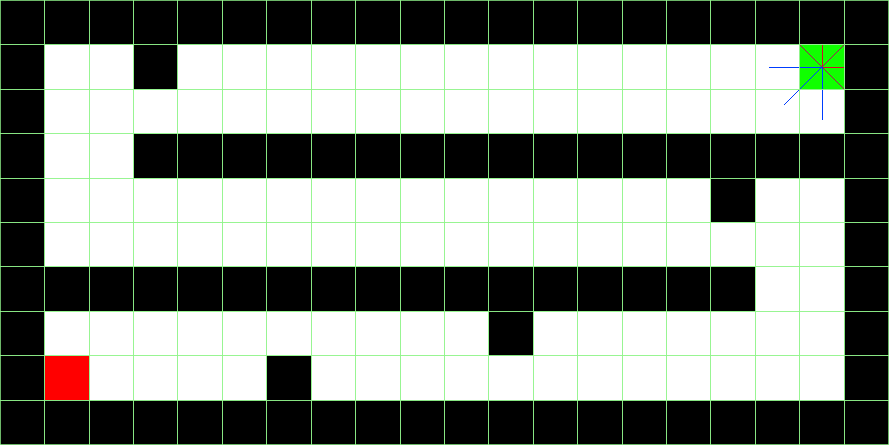
\includegraphics[width=10cm]{ruudukko_kuva.png}
\caption{Kaksiulotteinen neliöruudukko, jossa mustat ruudut ovat esteruutuja ja valkoiset ruudut vapaita ruutuja. Vihreä ruutu on aloitusruutu ja punainen ruutu on maaliruutu.}
\label{ruudukkokuva}
\end{figure}

Vähemmän tunnettuja pelialueen esitystapoja ovat kolmiointi ja kuusikulmiointi \parencite{abd2015comprehensive}. Alueen kolmiointi ja siihen perustuvat TA*- ja TRA*- algoritmit ovat kuitenkin osoittautuneet moninkertaisesti nopeammiksi suurissa pelialueissa verrattuna A*-algoritmiin \parencite{demyen2006efficient}. Kuusikulmioihin perustuvat pelialueet ja reitinhakualgoritmit ovat myös tuottaneet lupaavia tuloksia robotiikan tutkimuksessa sekä yleisesti suoriutuneet paremmin muistinkäytön ja ajankäytön suhteen verrattuna neliöruudukkoihin \parencite{abd2015comprehensive,lawande2022systematic}. Epäsäännöllisistä ruudukoista navigointiverkkoa on käytetty suurimmaksi osin videopeleissä ja esimerkiksi Unity tarjoaa dokumentaatiossaan laajat ohjeet ja menetelmät navigaatioverkon luomiseen \parencite{lawande2022systematic,unitydocnavmesh}.

\section{Reitinhakualgoritmit}

Graafin lyhimmän polun ongelmaa ja eri reitinhakualgoritmeja on tutkittu jo 1900-luvun puolivälistä lähtien. Vanhimmat ja tunnetuimmat algoritmit, Dijkstran algoritmi ja A*-algo\-rit\-mi, esiteltiin jo 50- ja 60-luvuilla ja ne pystyivät ratkaisemaan lyhimmän polun ongelman staattisessa graafissa \parencite{dijkstra1959note,hart1968formal}. Uudemmat reitinhaun sovellukset, kuten itseohjautuvat autot ja robotit, toivat kuitenkin alkuperäiselle ongelmanratkaisulle lisää vaatimuksia. Lyhimmän polun löytämisen lisäksi reitinhakualgoritmin täytyy ottaa huomioon sovelluksesta riippuen reitin turvallisuus, tehokkuus ja mahdollisten esteiden väistäminen \parencite{karur2021survey}.

A*-algoritmi on selvästi tunnetuin videopelien ja robottien reitinhaussa nopeutensa ansiosta \parencite{abd2015comprehensive,botea2013pathfinding,cui2011based}. A*-algoritmista on kehitetty jo monia eri variaatioita, jotka pyrkivät vastaamaan jatkuvasti kasvaviin vaatimuksiin. Tässä tutkimuksessa keskitytään tarkemmin A*-algoritmiin ja sen variaatioihin.

\subsection{A*-algoritmi}

A*-algoritmi on hyvin tunnettu paras-ensin-reitinhakualgoritmi, joka hyödyntää heuristista arviointifunktiota lyhimmän reitin etsimiseen \parencite{cui2011based,duchovn2014path}. A*-algoritmia voidaan pitää käytetyimpänä graafien etsintäalgoritmina etenkin videopeleissä \parencite{botea2013pathfinding,lawande2022systematic}.

Algoritmin toiminta tapahtuu seuraavasti: jokainen aloitussolmun vierekkäinen solmu arvioidaan kaavan \[f(n)=h(n)+g(n)\] mukaisesti, jossa \(n\) on solmu, \(h(n)\) on heuristinen etäisyys solmusta \(n\) maalisolmuun ja \(g(n)\) on todellinen etäisyys aloitussolmusta solmuun \(n\). Näistä solmuista matalimman \(f(n)\)-arvon solmu käsitellään seuraavaksi, jolloin kyseisen solmun vierekkäisten solmujen \(f(n)\)-arvot lasketaan. Tämä prosessi jatkuu, kunnes maalisolmu saavutetaan. Heuristiikan ollessa nolla A*-algoritmista tulee Dijkstran algoritmi.

A*-algoritmilla on \textcite{hart1968formal} mukaan kolme esitettyä ominaisuutta. Ensiksi A*-algoritmi löytää reitin, jos sellainen on olemassa. Toiseksi reitti on optimaalinen, jos heuristiikka on luvallinen eli arvioitu etäisyys on lyhyempi tai yhtä suuri kuin todellinen etäisyys. Viimeisenä mikään muu algoritmi samalla heuristiikalla ei käy läpi vähemmän solmuja kuin A*-algoritmi eli A* käyttää heuristiikkaa tehokkaimmalla mahdollisella tavalla \parencite{cui2011based,hart1968formal}. Luvallisia heuristiikkoja ovat solmujen vierekkäisyydestä riippuen Euklidinen etäisyys, Manhattan-etäisyys, Chebyshev-etäisyys ja Octile-etäisyys \parencite{botea2013pathfinding,duchovn2014path}. Manhattan-etäisyyttä käytetään pääasiassa neljän suunnan ja Octile- sekä Chebyshev-etäisyyttä kahdeksan suunnan vierekkäisyyksissä. Euklidista etäisyyttä voidaan käyttää tilanteessa, jossa agentti voi siirtyä seuraavaan soluun mistä kulmasta tahansa.

\subsection{A*-algoritmin variaatiot}
\label{avariaatiot}

Reitinhakualgoritmeja toteutettiin alunperin valmiisiin ja tarkkoihin ympäristöihin, joka ei kuitenkaan ole verrattavissa reaalimaailman tilanteisiin, joissa ympäristö voi muuttua arvaamattomasti \parencite{lawande2022systematic}. A*-algoritmia ja sen rajoitteita onkin tutkittu jo useita vuosikymmeniä, joka on mahdollistanut useiden eri variaatioiden kehittämisen. Useimmiten variaatiot keskittyvät korjaamaan yleisimpiä A*-algoritmin ongelmia, kuten tehokkuutta ja sopeutumista dynaamisiin alueisiin \parencite{stentz1994optimal}.

\textcite{stentz1994optimal,stentz1995focussed} esitti 90-luvulla kaksi A*-algoritmin variaatiota: D*-algoritmi (Dynamic A*) ja Focussed D*-algoritmi. Uudet variaatiot pyrkivät ratkaisemaan etenkin dynaamisen ja tuntemattoman alueen ongelmat robotiikan tutkimuksessa. Alkuperäinen D*-algoritmi teki mahdolliseksi reitin korjaamisen esteen tai muutoksen tullessa reitille. Focussed D*-algoritmi tehosti alkuperäisen D*-algoritmin toimintaa ajallisesti ja näin kehitti sen toimintaa entisestään.

\textcite{koenig2005fast} esittivät myöhemmin 2000-luvulla D* Lite -algoritmin, joka nimestään huolimatta ei varsinaisesti perustu suoraan D*-algoritmiin, vaan LPA* (Lifelong Planning A*) -algoritmiin. D* Lite -algoritmi osoittautui yksinkertaisemmaksi ja hieman tehokkaammaksi kuin D*- ja Focussed D*-algoritmit, jonka vuoksi sen toteuttaminen ja soveltaminen oli helpompaa. Tavoitteena oli luoda vahva perusta tulevalle tutkimukselle etenkin robotiikan parissa.

\section{Reitinhaun haasteet}

Yhden agentin staattisen ruudukkoalueen reitinhakuongelma on ratkaistavissa optimaalisesti heuristisilla reitinhakualgoritmeilla, mutta nykyään videopeleissä reitinhakuongelmat ovat monimutkaisempia ja saattavat vaatia useiden eri kriteerien täyttymisen. Suurimpia haasteita ovat esteiden järkevä väistäminen, optimaalisen reitin löytäminen ja suorituskykyvaatimusten minimointi \parencite{abd2015comprehensive,cui2011based}. Näiden lisäksi reitinhakuongelmat pitävät sisällään esimerkiksi useamman agentin samanaikaista reitinhakua ja reaaliajassa muuttuvan alueen reitinhakua. Siksi videopeleissä onkin käytössä monia eri reitinhakualgoritmeja, joista osa on kehitetty toimimaan dynaamisissa ympäristöissä, osa staattisissa ympäristöissä ja osa molemmissa \parencite{lawande2022systematic}. Reitinhakualgoritmin valinta on siis riippuvainen käyttötarkoituksesta. Nykytutkimus keskittyy pääasiassa monimutkaisten reitinhakuongelmien ratkaisemiseen ja algoritmien vertailuun erilaisissa reitinhakutilanteissa.

\subsection{Suorituskyky}

Reitinhakualgoritmin täytyy minimoida suorituskyvyn vaatimukset ja tallennustilan käyttö. Vaikka komponentit ovatkin kehittyneet vuosi vuodelta nopeasti, myös videopelit ovat monimutkaistuneet ja niiden laskennalliset vaatimukset kasvaneet. Reitinhakualgoritmeille varatut resurssit ovat videopeleissä rajatut, koska resursseja käytetään hyvin paljon myös graafisiin ja fysikaalisiin laskelmiin \parencite{lawande2022systematic}. Suorituskykyyn liittyen etenkin muistinkäyttöä ja laskentatehoa pidetään yleisesti rajoittavina tekijöinä videopelien reitinhaussa \parencite{botea2013pathfinding}. Ongelmia voidaan ratkaista erilaisilla algoritmeilla tai pelialueen esitystapaan liittyvillä ratkaisuilla \parencite{botea2013pathfinding,cui2011based}.

Yksi suorituskykyyn liittyvistä ongelmista on reitinhakualgoritmien huono skaalautuvuus etenkin muistinkäytön suhteen. Jos agentin reitinhakuun sovelletaan A*-algoritmia suurella 1000x1000 pelialueella, muistiin joudutaan tallentamaan pahimmassa tapauksessa miljoona solmua \parencite{cui2011based,duchovn2014path}. Muistinkäyttöä havainnollistetaan kuvassa \ref{astarmemory}, jossa A*-algoritmia on käytetty esteitä sisältävän alueen reitinhakuun. Kuvan keltaiset ruudut ovat tallennettu muistiin reitinhaun aikana. Kuvasta huomataan, että A*-algoritmi käy läpi suuren määrän ylimääräisiä solmuja, koska alueella on esteitä. Ongelma moninkertaistuu, jos alueella liikkuu useita reitinhakuagentteja. Tässä tapauksessa A*-algoritmi osoittautuu riittämättömäksi ongelman ratkaisemiseen, joten tilanteeseen kannattaa soveltaa erilaisia menetelmiä tai algoritmien variaatioita.

\begin{figure}[h]
\centering
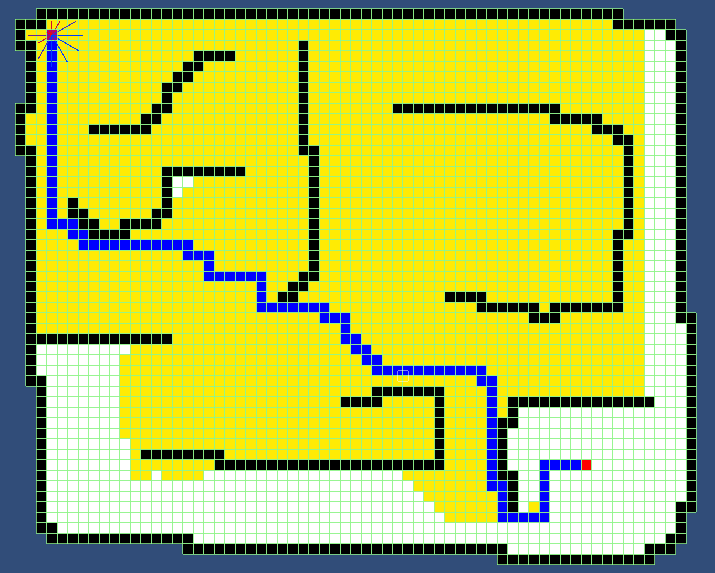
\includegraphics[width=10cm]{a_star_memory.png}
\caption{Kaksiulotteinen neliöruudukkoalue, jossa sininen reitti on A*-algoritmin laskema optimaalisin reitti. Keltaiset ruudut ovat käsitellyt solmut, jotka on tallennettu muistiin.}
\label{astarmemory}
\end{figure}

\subsection{Dynaamisen alueen reitinhaku}

Dynaamisen eli muuttuvan alueen reitinhaussa pyritään löytämään optimaalisin reitti jatkuvasti muuttuvassa alueessa \parencite{lawande2022systematic}. Dynaamisen alueen reitinhakua esiintyy erityisesti robotiikassa, mutta myös videopeleissä. Robottien reitinhaussa ympäröivää tilaa mitataan erilaisten sensorien avulla, jonka perusteella reitinhakua suoritetaan \parencite{rahmani2022towards}. Videopeleissä pelialue on usein valmiiksi reitinhakuagentin tiedossa eikä erillisiä sensoreita käytetä pelialueen havainnoimiseen, ellei erikseen haluta agentin toimivan täysin tuntemattomassa ympäristössä.

Videopeleissä pelialue voi muuttua toisten pelaajien, ei-pelaaja-hahmojen tai muuten vain liikkuvien esteiden takia. Esimerkiksi kilpa-ajoneuvopeleissä pelaaja voi kisata ei-pelaaja-hahmon kanssa, joka joutuu väistelemään sekä pelaajan ajoneuvoa että muita alueen liikkuvia esteitä \parencite{sazaki2017pathfinding}. Jokainen alueen muutos rikkoo reitinhakugraafin rakenteen, jolloin graafi ja valittu reitti täytyy korjata. Graafin luominen voi olla isoissa pelialueissa kallis operaatio, joten jatkuva uudelleenluominen ja uuden reitin etsiminen ei välttämättä ole vaihtoehto suorituskyvyn kannalta. Nykyään videopelien reitinhaun tutkimuksissa painotetaankin dynaamisia reitinhakualgoritmeja.

Graafin jatkuva päivittäminen on tuonut erilaisia ideoita tutkimuksissa. Luvussa \ref{avariaatiot} mainittu D*-algoritmi ja sen muunnelmat ovat kehitetty juuri tuntemattoman ja dynaamisen alueen reitinhakuun. Myös koneoppimismenetelmiä on alettu soveltamaan dynaamisissa alueissa. \textcite{lei2018dynamic} käyttivät syvää vahvistusoppimista koneoppimisagentin opettamiseen simulaatiossa ja testasi algoritmia myös reaalimaailman robotin reitinhaussa. Robotti käytti lidar-sensoreita lähiympäristön mallintamiseen ja onnistui muuttamaan reittiään esteiden tullessa eteen.

\subsection{Moniagenttireitinhaku}

Moniagenttireitinhaussa alueella on useampi kuin yksi agentti ja jokaisella niistä on oma aloitus- ja lopetuspisteensä graafissa. Jokaisella aika-askeleella agentti voi joko liikkua toiseen solmuun tai pysyä paikallaan nykyisessä solmussaan \parencite{sharon2015conflict,stern2019multi}. Tarkoituksena on samaan aikaan ratkaista moniagenttireitinhakuongelma ja minimoida reitinhaun kustannusfunktio (engl. cost function). Yleinen kustannusfunktio on \textit{sum-of-costs}, joka on agenttien aika-askelten summa kun ne saapuvat kohteisiinsa. Kustannusfunktiona voi olla myös \textit{makespan}, joka minimoi ajan kunnes viimeinen agentti on saapunut kohdesolmuun tai \textit{fuel}, joka minimoi agenttien kulkeman matkan. Erityinen huomio \textit{fuel}- kustannusfunktiossa on se, että paikallaan odottaminen ei nosta kustannusta.

Moniagenttireitinhaun rajoitteet voivat vaihdella tutkimusalasta riippuen, kuten esimerkiksi saavatko agentit kulkea samaa reittiä pitkin seuraten toisiaan, mutta yleensä perusrajoitteet ovat samat \parencite{sharon2015conflict,stern2019multi}. Perinteisesti agenttien täytyy liikkua lopetuspisteeseen törmäämättä toisiinsa matkalla eli ts. yhdellä solmulla ei saa olla samanaikaisesti enempää kuin yksi agentti. Kaksi agenttia eivät myöskään saa kulkea saman kaaren kautta samalla aika-askeleella. Moniagenttireitinhakuongelman sovelluksia esiintyy videopelien lisäksi esimerkiksi robotiikassa, ilmailussa, liikennesuunnittelussa ja itseohjautuvissa ajoneuvoissa, joten se on saanut viime vuosina paljon huomiota tutkimuksissa ja akateemisissa yhteisöissä.

Moniagenttireitinhakuongelmaan on sekä optimaalisia että epäoptimaalisia ratkaisuja \parencite{sharon2015conflict}. Optimaaliset ratkaisut ovat luonteeltaan NP-kovia, koska agenttien lukumäärä kasvattaa ongelman tila-avaruutta eksponentiaalisesti. A*-algoritmi on esimerkiksi optimaalinen ratkaisu, mutta moniagenttireitinhaussa sen suoritusaika voi olla hyvin pitkä ja muistinkäyttö liian suurta. Tämän vuoksi ongelmissa, joissa agentien lukumäärä on suuri, käytetään usein epäoptimaalisia ratkaisuja.

\chapter{Koneoppiminen}
\label{koneoppiminen}

Koneoppiminen on tällä hetkellä yksi teknisten tutkimusalojen suosituimmista aihealueista. Sen ydin rakentuu kysymykselle, pystyykö tietokone jäljittelemään ihmismielen oppimisprosessia ja täten oppia automaattisesti kokemuksen kautta \parencite{das2017survey,jordan2015machine}. Automaattisella oppimisella pyritään vähentämään manuaalista, tapaus tapauksen perään ohjelmoimista. Sen sijaan konetta opetetaan syöte-tuloste-parien avulla. Vuosikymmenten aikana koneoppimisen tutkimus on edistynyt merkittävästi eikä loppua ole toistaiseksi näkyvissä. Uudet sovellukset ja algoritmit, laskentatehon kasvu ja massadata (engl. big data) eli hyvin suuret, keskittyneet datamäärät ovat tuoneet tarpeen sekä teorian tutkimukselle että kehittyneille käytännön ratkaisuille.

\section{Koneoppimisen perusteet}

Koneoppiminen on tieteenalana yhdistelmä tietotekniikkaa ja tilastotieteitä. Tietotekniikka ja tietokoneet mahdollistavat ongelmanratkaisun. Suurista datajoukoista oppiminen, erilaisten ennusteiden tekeminen ja päätöksenteko vaativat sen sijaan tilastotieteellisiä menetelmiä \parencite{das2017survey,jordan2015machine}. Myös neurotieteiden ja psykologian roolit ovat kasvamassa koneoppimisen tutkimuksessa. Esimerkiksi ihmisaivojen ja sitä kautta oppimisprosessin tutkiminen ja hyödyntäminen koneoppimisessa ovat tulevaisuudessa merkittäviä tutkimuksen kohteita \parencite{das2017survey}. Koneoppimisen sovellukset ovat nykyään hyvin laaja-alaiset. Tunnettuja esimerkkejä ovat konenäkö, puheentunnistus ja robotiikka. Konenäköä hyödynnetään etenkin terveydenhoidon alalla anomalioiden tunnistamiseen kuvissa. Mainonnassa koneoppimista käytetään personoitujen suositusten luomiseen ja markkinoinnissa erilaisissa ennusteissa.

Tietoteknisten laitteiden suosio ja sitä kautta datan räjähdysmäinen kasvu ovat olleet suuressa roolissa koneoppimisen hyödyntämisessä. Massadataa on mahdotonta tarkastella manuaalisesti, joten niiden käsittelyyn on otettu käyttöön koneoppimisen menetelmiä \parencite{jordan2015machine}. Koneoppimisalgoritmit pystyvät muokkaamaan palveluita vastaamaan jokaisen henkilökohtaisiin tarpeisiin personoidun datan avulla. Esimerkiksi mainoksia voidaan kohdentaa tietyille ryhmille ja vanhoja potilastietoja voidaan hyödyntää hoitotyypin valitsemiseen tietyille potilaille. Personoitu data tuo tosin myös tietoturvallisia haasteita. Henkilödatasta on pyrittävä tekemään anonyymia, jottei sitä pysty yhdistämään suoraan henkilöihin. Samalla kuitenkin data voi olla niin tarkkaa, että jokaisella sanotaan olevan oma digitaalinen sormenjälki suuressa datamassassa. Myös suorituskykyvaatimukset ovat nousseet datan kasvun myötä, joten algoritmit täytyy kehittää mukautuviksi.

Koneoppiminen perustuu koneen opettamiseen erillisen opetusdatan avulla \parencite{das2017survey,jordan2015machine}. Opetusdatasta pyritään havaitsemaan piilossa olevia malleja tilastotieteellisten menetelmien avulla. Kohdatessaan uusia esimerkkejä ja uutta dataa kone pystyy muodostamaan arvion vastauksesta havaitun mallin perusteella. Opetusdata voi olla valmiiksi luokiteltua tai kokonaan luokittelematonta, joista luokiteltua dataa käytetään tavallisesti ohjattuun oppimiseen perustuvissa menetelmissä ja luokittelematonta dataa ohjaamattomaan oppimiseen perustuvissa menetelmissä.

Koneoppimisella yritetään perinteisesti ratkaista luokitteluongelmia, joissa datajoukosta voidaan päätellä, kuuluuko käsiteltävä asia tiettyyn luokkaan vai ei \parencite{jordan2015machine}. Esimerkiksi sähköposti voidaan luokitella roskapostiksi tai aidoksi sähköpostiksi riippuen mitkä ovat luokittelun vaihtoehdot. Koneoppimisen avulla kasvatetaan luokittelun tarkkuutta, joka on kyseisen luokitteluongelman tärkein mittari. Opetusdata voi koostua kokoelmasta erilaisia sähköposteja, jotka on valmiiksi luokiteltu roskapostiksi tai aidoksi sähköpostiksi. Syötteenä on siis yksittäinen sähköposti ja tulosteena roskaposti tai aito. Koneoppimisen avulla kone opetetaan tunnistamaan malleja ja kuvioita datassa, jolloin se pystyy myöhemmin tunnistamaan samoja kuvioita oikeissa tilanteissa.

\section{Koneoppimisen paradigmat}

Koneoppiminen voidaan jakaa eri osiin oppimistyylin mukaan. Oppimistyylejä ovat esimerkiksi ohjattu oppiminen, puoliohjattu oppiminen, ohjaamaton oppiminen, transduktio ja vahvistusoppiminen \parencite{das2017survey}. Näistä tunnetuimpia ovat ohjattu oppiminen, ohjaamaton oppiminen ja vahvistusoppiminen.

\subsection{Ohjattu oppiminen}

Käytetyin oppimistyyli on ohjattu oppiminen ja siihen liittyvät menetelmät \parencite{jordan2015machine,nasteski2017overview}. Ohjatun oppimisen tehtävät voidaan jakaa luokitteluun ja regressioon. Luokitteluongelmissa vastaukset ovat kategorisia, esimerkiksi lintu, koira tai jokin kokonaisluku, ja regressiossa jatkuvia lukuarvoja, esimerkiksi hinta. Ohjatussa oppimisessa opetusaineisto tuodaan \((x,y)\) pareina, jossa \(x\) on syöte ja \(y\) on tulos. Oppijan tavoitteena on approksimoida funktio, joka kuvaa kaikki syötteet niitä vastaaviin tuloksiin. Yksittäisessä luokittelutehtävässä oppija luo mahdollisimman tarkan ennusteen \(y\) syötteen \(x\) perusteella ja vertaa ennustetta oikeaan tulokseen. Jos ennuste on väärä, niin mallia muokataan tarpeen mukaisesti. Yleisesti ohjatun oppimisen heikkoutena voidaan pitää luokitellun datan saatavuutta ja laatua \parencite{das2017survey}. Data täytyy esikäsitellä ja luokitella ennalta muilla menetelmillä, joka nostaa lopullista laskentakustannusta. Toisaalta jotkin menetelmät, kuten naiivi Bayes-luokittelija, eivät vaadi suuria datamääriä tuottaakseen tarkkoja vastauksia \parencite{osisanwo2017supervised}. Naiivi Bayes -luokittelijan lisäksi tunnettuja ratkaisualgoritmeja ovat päätöspuut ja tukivektorikoneet.

Päätöspuu (engl. decision tree) on tiedonlouhinnassa ja koneoppimisessa käytetty luokittelualgoritmi, jolla luokitellaan asioita ominaisuuksien perusteella \parencite{nasteski2017overview,osisanwo2017supervised}. Päätöspuu koostuu juurisolmuista, oksasolmuista ja lehdistä. Juuri- ja oksasolmuissa sijaitsee yksittäisiä piirteitä ja lehtisolmuissa mahdollisia tuloksia. Luokittelu alkaa juurisolmusta ja päätyy johonkin lehtisolmuun eli yksittäiseen tulokseen. Tarvittaessa päätöspuun yleistä arviointi- ja suorituskykyä voidaan parantaa karsimalla (engl. prune). Karsimisessa päätöspuun tarpeettomia solmuja poistetaan kokonaan käytöstä, jolla vähennetään esimerkiksi ylisovittamista.

Naiivi Bayes -luokittelija (engl. naive-Bayes) on ohjatussa oppimisessa käytetty luokittelumenetelmä, jolla luokitellaan asioita piirteiden perusteella käyttäen Bayesin todennäköisyysteoreemaa \parencite{nasteski2017overview,rish2001empirical}. Yksinkertaistamisen vuoksi naiivi Bayes -luo\-kit\-te\-li\-jas\-sa piirteet oletetaan tilastollisesti riippumattomiksi toisistaan, jolloin tuloksena saadaan approksimaatio luokittelusta. Tästä huolimatta naiivi Bayes -luokittelija on osoittautunut tehokkaaksi menetelmäksi käytännön luokitteluongelmissa, kuten tekstin luokittelussa ja lääketieteellisessä diagnosoinnissa \parencite{rish2001empirical}.

Tukivektorikone (engl. support vector machine, SVM) on yksi tunnetuimmista ja tehokkaimmista ohjatun oppimisen menetelmistä luokitteluun ja regressiotehtäviin \parencite{cervantes2020comprehensive,osisanwo2017supervised}. Opetusaineistosta saaduista ominaisuuksista muodostetaan piirreavaruus (engl. feature space), josta luokat erotellaan toisistaan piirteiden perusteella. Luokkia erottelevaa rajapintaa kutsutaan tasoksi (engl. plane) ja etäisyyttä tasoa lähimpänä olevaan datapisteeseen marginaaliksi (engl. margin). Kaksi vektoria, jotka kulkevat tason molempien puolien lähimpien pisteiden kautta, muodostetaan yksisuuntaisesti tasoon nähden ja näiden vektorien etäisyys toisistaan pyritään maksimoimaan, jolloin tavoitteena on minimoida luokitteluvirhe ja parantaa yleistämistä.

\subsection{Ohjaamaton oppiminen}

Ohjaamattomassa oppimisessa analysoidaan luokittelematonta dataa \parencite{das2017survey,jordan2015machine}. Tarkoituksena on tehdä päätelmiä datan rakenteesta ja malleista ilman ulkopuolista ohjeistusta. Erityisen tärkeää on pyrkiä valitsemaan datasta ominaispiirteet, jotka ovat relevantteja datan tarkastelun kannalta. Liian suuri määrä piirteitä kasvattavat datajoukon ulottuvuutta eli dimensiota ja näin ollen tekee datajoukon rakenteesta monimutkaisen. Datajoukkoa pyritään strukturoimaan eri menetelmien avulla, jolloin datan tarkastelua pyritään selkeyttämään. Klusterointi ja dimension redusointimenetelmät ovat yleisiä datan strukturointimenetelmiä.

Klusteroinniksi kutsutaan menetelmiä, joissa datapisteet jaetaan ominaispiirteidensä perusteella klustereihin \parencite{usama2019unsupervised}. Yksittäiset klusterit sisältävät siis ominaisuuksiltaan samankaltaiset datapisteet. \textit{K-means} -klusterointi on tunnettu klusterointimenetelmä, jossa datapisteet \(n\) jaetaan \(K\):hon klusteriin. Klusterin keskipistettä lähimpänä oleva datapiste toimii eräänlaisena prototyyppinä, johon muiden datapisteiden etäisyyksiä verrataan. Uusi datapiste katsotaan kuuluneeksi siihen klusteriin, jonka keskipisteeseen on pienin etäisyys.

Dimension redusointimenetelmät pyrkivät tihentämään datajoukkoa ja helpottamaan sen analysointia \parencite{usama2019unsupervised}. Niiden periaatteena on vähentää datajoukossa tarkasteltavia ominaispiirteitä ja näin ollen vähentää datajoukon kokonaisulottuvuutta, jolloin datajoukon analysointi yksinkertaistuu. Uuteen datajoukkoon pyritään sisällyttämään keskeisimmät piirteet siten, ettei relevanttia informaatiota katoaisi. Pääkomponenttianalyysi on yksi tunnetuimmista ja vanhimmista dimension redusointimenetelmistä, jossa olemassaolevasta datajoukosta poimitaan tärkeimmät piirteet ja niistä luodaan pääkomponentteja (engl. principal components) \parencite{abdi2010principal}.

\subsection{Vahvistusoppiminen}

Vahvistusoppiminen on kolmas suuri koneoppimisen paradigma, jossa oppijana toimii agentti ja agentin toimintaa ohjaavat palkkiot \parencite{arulkumaran2017brief,jordan2015machine,li2018deep}. Vahvistusoppimisen opetusaineisto eroaa muiden paradigmojen opetusaineistoista siten, ettei tietylle syötteelle \(x\) anneta valmiiksi oikeaa tulosta \(y\) tai etsitä rakenteellisia malleja datajoukosta, vaan agentti saa jokaisesta suorittamastaan toiminnosta positiivisen tai negatiivisen palkkion. Palkkiot ohjaavat agentin oppimisprosessia ja käyttäytymistä ympäristössä. Toimintojen ja niistä saatujen palkkioiden lisäksi agentti on jatkuvassa vuorovaikutuksessa ympäristönsä kanssa siten, että agentti tarkkailee toimintojensa vaikutuksia ja ympäristön tilamuutoksia. Näin agentti pystyy muokkaamaan toimintojaan saamiensa palkkioiden perusteella. Vahvistusoppimistehtävän ideaaliratkaisu on palkkiot maksimoivan käytännön (engl. policy) selvittäminen. Käytäntöä voidaan pitää todennäköisyytenä tehdä tietty toiminto tietyssä tilassa ja kyseistä todennäköisyyttä päivitetään saatujen palkkioiden avulla. Esimerkiksi reitinhaussa kohteeseen pääseminen tuo agentille positiivisen palkkion, jolloin agentti kasvattaa todennäköisyyttä valita tila-toiminto-pareja, jotka veivät sen kohteeseen.

Vahvistusoppiminen voidaan kuvata Markovin päätösprosessina (engl. Markov decision pro\-cess) tilojen \(S\), toimintojen \(A\) ja palkkiosignaalien \(r\) avulla \parencite{arulkumaran2017brief}. Jokaisella aika-askeleella \(t\) agentti suorittaa toiminnon \(a\), jolloin ympäristön tila \(s\) muuttuu ja muutos viestitään agentille palkkiosignaalin \(r\) kautta. Palkkiosignaalin lisäksi ympäristö viestii agentille tilamuutoksesta, jolloin agentti saa tiedon uudesta tilasta \(s\) + 1. Palkkion ja uuden tilan perusteella agentti valitsee jälleen seuraavan toimintonsa. Markov-prosessi voi olla jaksollinen (engl. episodic), jolloin tila nollaantuu tietyn ajan jälkeen. Agentin lopullisena tavoitteena on saavuttaa paras mahdollinen käytäntö, joka maksimoi saadun palkkion määrän. Kuva \ref{reinflearning} havainnollistaa vahvistusoppimisen toimintaa.

\begin{figure}[h]
\centering
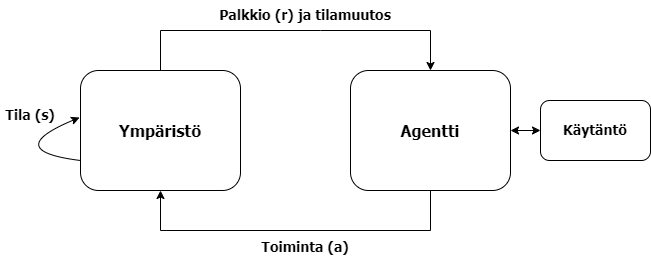
\includegraphics[width=13.5cm]{reinflearning.png}
\caption{Vahvistusoppimisympäristön oppimissilmukka yhdellä aika-askeleella.}
\label{reinflearning}
\end{figure}

Oppiakseen optimaalisen käytännön agentin tekemät päätökset vaativat jonkin ennusteen tulevien toimintojen arvosta. Yleisesti tämän ennusteen laskemista kutsutaan nimellä \textit{action-value function}, ja yksi tunnettu menetelmä sen laskemiseen on Q-oppiminen (engl. Q-lear\-ning). Q-oppiminen on mallivapaa menetelmä eli se ei tarvitse toimiakseen erillistä mallia ympäristöstä. Q-oppimisessa jokaisen tilan eri toimintoa arvioidaan \textcite{arulkumaran2017brief} esittämän kaavan \[Q(s,a) = r_t + \gamma max_a Q^\pi (s_{t+1},a)\] mukaisesti, jossa \(s\) on tila, \(a\) on toiminto, \(r_t\) on tilan palkkio, $\gamma$ on erillinen alennusparametri, joka määrittää tulevien toimintojen tärkeyden aiempiin verrattuna ja \(max_a Q^\pi (s_{t+1},a)\) on ennakkoarvio tulevasta, optimaalisesta palkkiosta.

Funktiosta saatuja arvoja päivitetään erillisessä Q-taulussa. Oppimisepisodien aikana agentti pystyy ennakoimaan Q-taulun avulla jokaisen mahdollisen toimintonsa tulevaa lopullista palkkiota ja tarvittaessa päivittämään Q-taulun arvoja. Ongelmaksi osoittautuu kuitenkin uuden tutkimisen (engl. exploration) ja olemassa olevan tiedon hyödyntämisen (engl. exploitation) tasapainotus \parencite{arulkumaran2017brief}. \textit{Epsilon-Greedy} on menetelmä, jossa tietyllä todennäköisyydellä $\epsilon$ agentti valitsee pienemmän arvon tilan, jolloin voidaan löytää uusia ja parempia ratkaisuja tavoiteltuun lopputulokseen \parencite{li2018deep,panov2018grid}. Agentti voi myös jatkaa aiemman käytännön hyödyntämistä todennäköisyydellä 1 - $\epsilon$.

Vahvistusoppimiseen liittyy haasteita optimaalisen käytännön löytämisessä ja agentin satunnaisissa toiminnoissa \parencite{arulkumaran2017brief}. Optimaalinen käytäntö on mahdollista löytää vain jatkuvan yrittämisen kautta, ja ainoana oppimisen signaalina toimivat saadut palkkiot. Riippuen tehtävän haastavuudesta lukuisatkaan yritykset eivät välttämättä takaa optimaalista ratkaisua. Toiseksi agentin palkkioon johtavissa toiminnoissa saattaa olla paljon turhia toimintoja eli toisin sanoen agentti ei välttämättä tiedä, mitkä toiminnot oikeasti johtivat palkkion saamiseen. Esimerkiksi robotin liikkuessa sisätiloissa sen havainnot riippuvat vahvasti siitä, kohtaako se matkalla umpikujia vai siirtyykö se satunnaisilla toiminnoilla suoraan kohteeseen. Jos palkkio annetaan maaliin pääsemisen yhteydessä, niin robotti voi olettaa, että umpikujaan päätyminen kuului palkkion saamiseen vaativien toimintojen joukkoon. Tätä ongelmaa kutsutaan nimellä \textit{(temporal) credit assignment problem}.

\section{Syväoppiminen}

Koneoppimisen ja sitä kautta myös syväoppimisen tutkimus on ollut viime vuosina hyvin aktiivista \parencite{pouyanfar2018survey}. Syväoppimisella ollaan onnistuttu ratkaisemaan ongelmia, joita tekoälyn tutkimuksessa on yritetty ratkaista jo vuosia \parencite{lecun2015deep,pouyanfar2018survey}. Erityisesti tuloksia on tullut kuvantunnistuksessa, puheentunnistuksessa ja erilaisissa luonnollisen kielen prosessoinnin tehtävissä. Merkittävimpiä syväoppimisen tutkimuksen keksintöjä viime vuosikymmenillä ovat vastavirta-algoritmi (engl. backpropagation), konvoluutioneuroverkon (engl. Convolutional Neural Network, CNN) inspiraationa tunnettu neocogitron-neuroverkko, siitä hieman myöhemmin kehitetty takaisinkytketty neuroverkko (engl. Recurrent Neural Network, RNN) ja syvä uskomusverkko (engl. Deep Belief Network, DBM). Syvä uskomusverkko mahdollisti entistä syvemmän neuroverkon oppimisen, jonka seurauksena siirryttiin yleisesti käyttämään termiä syväoppiminen. Viime vuosien yksi tunnetuimpia syväoppimisen sovelluksia on Googlen AlphaGo, joka onnistui päihittämään useita Go-pelin ammattilaisia pelin äärimmäisestä strategisesta haastavuudesta huolimatta. Tässä luvussa kerrotaan neuroverkkojen, syväoppimisen ja syvän vahvistusoppimisen toiminnan perusteet sekä esitellään Soft Actor-Critic -algoritmi, jota myöhemmin sovelletaan tutkimuksen empiirisessä osuudessa.

\subsection{Neuroverkkojen perusteet}

Neuroverkkojen perusosiin kuuluvat perseptronit (engl. perceptron), jotka ovat keinotekoisia neuroneita \parencite{nielsen2015neural}. Perseptronit koostuvat binäärisistä syötteistä \(x_{1}, x_{2}, x_{3},..,\) ja yksittäisestä binäärisestä tuloksesta. Syötteiden relevanttius määritellään erillisten painoarvojen (engl. weight) \(w_{1}, w_{2}, w_{3},..,\) perusteella. Syötteet ja painoarvot lasketaan painotettuna summana $\sum_{j}w_{j}x_{j}$ ja tulokseen lisätään neuronin vakiotermi (engl. threshold tai bias), joka on neuronille parametrina annettu luku ja määrittää onko lopullisena tuloksena 0 vai 1. Yksinkertaistettuna \textcite{nielsen2015neural} kuvaa perseptronia "laitteeksi, joka tekee päätökset punnitsemalla todisteita".

Yleisesti neuroverkko koostuu syötekerroksesta, piilokerroksesta ja ulostulokerroksesta \parencite{nielsen2015neural}. Piilokerros koostuu yhdestä tai useammasta perseptroni-kerroksesta. Ensimmäisellä perseptroni-kerroksella tehdään yksinkertaisimmat päätökset ja jokaisella seuraavalla kerroksella tehdään toinen toistaan monimutkaisempia päätöksiä. Kerrosten suuri lukumäärä mahdollistaa siis vaativienkin päätösten tekemisen.

Oppiminen on mahdollista painoarvoja muuttamalla, jolloin koko neuroverkon lopullinen tulos muuttuu \parencite{nielsen2015neural}. Vaarana kuitenkin on, että pienet muutokset muuttavat neuroverkon tulosta radikaalisti vastakkaiseen suuntaan. Korvaamalla alkuperäiset, binääriset perseptronit Sigmoid-neuroneilla painoarvojen muutokset eivät aiheuta suurta muutosta tuloksessa. Sigmoid-neuronit käyttävät sigmoid-funktiota porrasfunktion sijaan, jolloin tulos voi olla mitä tahansa 0 ja 1 välillä.

Kuten koneoppimisessa, myös syväoppimisessa neuroverkon opettaminen tapahtuu opetusaineiston avulla \parencite{nielsen2015neural}. Luokitteluongelman suoran ratkaisemisen sijaan neuroverkon opettamisessa keskitytään ensin painoarvojen ja vakiotermien muodostaman virhefunktion minimiarvon selvittämiseen ja vasta sen jälkeen luokittelun tarkkuuteen. Virhefunktion minimin löytämiseen käytetään tunnettua optimointikeinoa, gradienttimenetelmää (engl. gradient descent) ja vastavirta-algoritmia (engl. backpropagation). Vastavirta-algoritmilla voidaan laskea kerralla gradienttimenetelmään tarvittavat osittaisderivaatat painoarvojen ja vakiotermien suhteen virhefunktiossa. Tuloksena saadaan virhefunktion gradientti, jonka jälkeen painoarvot ja vakiotermit päivitetään neuroneissa takaperin iteroiden viimeisestä kerroksesta lähtien ja menetelmä toistetaan.

Gradienttimenetelmällä pyritään yleisellä tasolla selvittämään virhefunktion minimi suorittamalla pieniä askeleita kohti globaalia tai lokaalia minimiä \parencite{nielsen2015neural}. Askeleiden pituus määritellään oppimisnopeudella (engl. learning rate), joka on usein pieni vakioluku. Oppimisnopeus ei saa kuitenkaan olla liian pieni, koska muuten algoritmi toimii hyvin hitaasti. Oppimisnopeutta voidaan tehostaa myös käyttämällä stokastista gradienttimenetelmää, jossa painoarvot ja vakiotermit päivitetään vasta pienen opetusaineistojoukon jälkeen. Tästä saatu tulos toimii hyvänä arviona todelliselle gradienttivektorille.

\subsection{Syväoppimisen haasteet}

Yksi suurimmista syväoppimisen haasteista on ylisovittaminen (engl. overfitting) \parencite{nielsen2015neural}. Ylisovittamisessa neuroverkko oppii opetusaineiston liiankin täsmällisesti ja menettää sen johdosta kykynsä yleistää oppimaansa toisiin tapauksiin esimerkiksi testiesimerkkidatassa. Ylisovittamista ilmenee usein jos opetusaineiston luokittelun tarkkuus nousee lähelle sataa prosenttia, mutta testiesimerkkidatan luokittelun tarkkuus pysyy ennallaan. Ylisovittamista voidaan estää esimerkiksi neuroverkon pienentämisellä tai opetusaineiston kasvattamisella. Joskus opettaminen voidaan myös keskeyttää, jos testiesimerkkidatan tarkkuus ei tunnu enää kasvavan.

Ylisovittamista voidaan hillitä myös säännöstelyllä (engl. regularization), jossa pyritään pienentämään neuronien painoarvoja virhefunktion minimin löytämiseen \parencite{nielsen2015neural}. Suurten painoarvojen pienet muutokset voivat aiheuttaa suuria muutoksia neuroverkon toimintaan, jolloin se voi ajautua ylisovittamaan opetusaineistoa. Säännöstely toisin sanoen tehostaa neuroverkon kykyä tehdä yleistyksiä. Yleisiä säännöstelymenetelmiä ovat L1- ja L2-säännöstelyt sekä neuronien poistaminen (engl. dropout). Neuronien poistaminen eroaa muista mainituista siten, ettei siinä keskitytä virhefunktion muokkaamiseen, vaan neuroverkon piilokerroksesta poistetaan hetkellisesti neuroneita. Neuroverkon toiminta pysyy muuten ennallaan, mutta vain osaa neuroneista käytetään ja niiden parametreja päivitetään. Seuraavalla iteraatiolla neuronit palautetaan ja jälleen osa piilokerroksen neuroneista poistetaan väliaikaisesti. Jokainen iteraatio käyttää opettamiseen rakenteeltaan erilaista neuroverkkoa, koska osa neuroneista on piilotettu. Tämän avulla saadaan luotua tilanne, jossa samaa neuroverkkoa opettaessa opetetaankin useita erilaisia neuroverkkoja ja näiden neuroverkkojen ylisovittamiset kumoavat toisensa.

\section{Syvä vahvistusoppiminen}

Yksi tekoälyn tutkimuksen suurimpia tavoitteita on luoda täysin autonominen ja ohjailtava agentti, joka pystyy toimimaan erilaisissa ympäristöissä samalla oppien ja kehittäen käyttäytymistään paremmaksi \parencite{arulkumaran2017brief}. Alunperin vahvistusoppimisella pystyttiin kehittämään oppivia agentteja, mutta ongelmaksi osoittautui ongelmien ja ratkaisujen suppeus, koska pelkällä vahvistusoppimisella ei pystytty käsittelemään ja hyödyntämään moniulotteista dataa, kuten robotin raakaa sensoridataa tai kuvan pikseleitä. Syväoppimisella onnistuttiin vastaamaan tähän vaatimukseen, ja pian syvän vahvistusoppimisen sovelluksilla pystyttiin jo pelaamaan Atari 2600:n videopelejä käyttämällä hyväksi kuvan pikselidataa.

\subsection{Syvän vahvistusoppimisen menetelmät}

Syvä vahvistusoppiminen hyödyntää syväoppimista ja neuroverkkoja suurten tila- ja havaintoavaruuksien tapauksissa \parencite{arulkumaran2017brief,li2018deep}. Se eroaa vahvistusoppimisesta pääasiassa funktioapproksimaation suhteen. Esimerkiksi tavallisessa Q-oppimisessa muodostetaan taulu tila-toiminta-pareista ja niiden Q-arvoista, mutta syvässä Q-oppimisessa (engl. deep Q-learning) taulu korvataan neuroverkolla. Syvässä Q-oppimisessa tila, esimerkiksi pikselidata, syötetään neuroverkolle ja tuloksena saadaan mahdolliset toiminnot. Oppiminen tapahtuu neuroverkon tapaisesti eli tuloskerrokselta saatu tieto palkkiosta viedään vastavirta-algoritmilla takaisin syötekerrosta kohti ja samalla neuronien painoarvoja päivitetään. Esimerkiksi reitinhaussa agentti saa positiivisen palkkion saavuttaessaan kohteen, jolloin kohteeseen johtavia tila-toiminto-pareja pyritään valitsemaan todennäköisemmin päivittämällä neuroverkon painoarvoja. Syvässä Q-verkossa voi muodostua epävakautta, jolloin pienetkin muutokset Q-verkkoon voivat muuttaa käytäntöä merkittävästi \parencite{mnih2015human}. Tätä epävakautta voidaan korjata \textit{Experience replay}-menetelmällä. Menetelmässä tallennetaan muistiin satunnaisesti aiempia kokemuksia, joita agentti voi myöhemmin käyttää oppimiseen. Menetelmän hyöty perustuu siihen, että opettamisesta pyritään poistamaan ajalliset korrelaatiot.

Arvofunktioiden approksimaation perustuvat menetelmät kohtaavat suuria haasteita moniulotteisissa tila- ja toimintoavaruuksissa, kuten robotiikassa esiintyvissä ongelmissa on tapana olla \parencite{arulkumaran2017brief,deisenroth2013survey}. Vaihtoehtoisina menetelminä ovat \textit{policy search} -menetelmät, joissa arvofunktiomallin ylläpitämisen sijaan käytetään parametrisoituja käytäntöjä. Parametreja päivittämällä pyritään maksimoimaan odotettu tulos ja löytämään paras käytäntö. Policy search -menetelmät voivat olla mallipohjaisia tai mallivapaita eli joko ylläpidetään mallia ympäristöstä tai opetellaan suoraan käytäntö. Usein käytännön opetteleminen on helpompaa kuin tarkan mallin oppiminen.

Arvofunktioita ja policy search -menetelmiä voidaan hyödyntää myös yhdessä, jolloin saadaan tekijä-kriitikko-menetelmiä (engl. actor-critic) \parencite{arulkumaran2017brief}. Tässä kontekstissa sana tekijä viittaa käytäntöön ja kriitikko arvofunktioon. Tekijä käyttää kriitikolta saamaa palautetta oppimiseen tai toisin sanoen tekijä saa ympäristöltä tilan ja valitsee sen perusteella toiminnon ja samaan aikaan kriitikko saa ympäristöltä tilan ja edellisen aika-askeleen palkkion. Kriitikko laskee tämän perusteella ennustevirheen (engl. temporal difference) ja päivittää itsensä ja tekijän.

\subsection{Soft Actor-Critic}

Soft Actor-Critic (SAC) on \textcite{haarnoja2018soft} kehittämä mallivapaa ja \textit{off-policy} syvään vahvistusoppimiseen perustuva algoritmi. Off-policy tarkoittaa oppijan kykyä käyttää aiempaa dataa nykyisiin tehtäviin. Se kehitettiin vastaamaan yleisiin vahvistusoppimisalgoritmien ongelmiin reaalimaailmassa, kuten opetusaineiston kompleksisuuteen (engl. sample complexity) ja hyperparametrien herkkyyteen \parencite{haarnoja2018app}. Yksinkertaisetkin tehtävät saattoivat vaatia satoja tuhansia ellei jopa miljoonia opetusaskeleita ennen kuin hyväksyttävä lopputulos saavutettiin. Tämän lisäksi eri tehtävien välillä joutui virittelemään monien eri hyperparametrien arvoja, jotta oppiminen olisi edes mahdollista. SAC pyrkii mahdollisimman satunnaisiin toimintoihin samalla maksimoiden odotetun palkkiosumman, jota kutsutaan myös nimellä \textit{maximum entropy}. Tavallisesti parhaimman käytännön löytämisessä halutaan maksimoida saatu palkkio, mutta maximum entropy -periaatteessa yhtälöön lisätään erillinen entropia-termi. Entropian suuruutta kontrolloidaan kertoimen $\alpha$ avulla, jota kutsutaan myös lämpötilaksi (engl. temperature). Kerroin voidaan asettaa myös nollaksi, jolloin yhtälö palauttaa jälleen maksimipalkkion antavan käytännön.

Optimaalisen lämpötilan valitseminen on hankalaa useiden erilaisten tehtävien tapauksessa \parencite{haarnoja2018app}. Palkkion suuruus ja sitä kautta käytännön kehittyminen vaikuttavat optimaaliseen entropiaan ja siten myös lämpötilan valintaan. Kiinteän lämpötilan valitseminen ei ole kannattavaa, koska agentin tulisi pyrkiä etsimään uusia tiloja myös alueilta, joissa optimaalisista toiminnoista ei ole varmuutta. Toisaalta agentin tulisi myös pitää kiinni selvästi hyvistä tiloista ja toiminnoista. Ongelma ratkaistaan päivittämällä lämpötilatermiä siten, että käytännön entropian keskiarvo pysyy samana, mutta tilojen erilliset entropiat voivat vaihdella. Tähän käytetään apuna myös dynaamista ohjelmointia, jossa ongelma jaetaan pienempiin osiin ratkaisemista varten.

SAC suoriutui \textcite{haarnoja2018app} suorittamista testeistä selvästi nopeammin verrattuna muihin algoritmeihin, kuten PPO (proximal policy optimization), DDPG (deep deterministic policy gradient) ja TD3 (twin delayed deep deterministic policy gradient). Etenkin haastavat tehtävät osoittautuivat nopeammiksi ja lopputulokseltaan paremmiksi.

\chapter{Unity}
\label{unity}

Unity on Unity Technologiesin kehittämä pelinkehitysalusta, joka sisältää oman renderöinti- ja fysiikkamoottorin sekä Unity Editor -nimisen graafisen käyttöliittymän \parencite{juliani2018unity}. Unityllä on mahdollista kehittää perinteisten kolmiulotteisten ja kaksiulotteisten pelien lisäksi myös esimerkiksi virtuaalitodellisuutta (engl. virtual reality) hyödyntäviä pelejä tietokoneille, mobiililaitteille ja pelikonsoleille. Unitystä onkin vuosien mittaan tullut yksi tunnetuimmista pelinkehitysalustoista, jonka parissa työskentelee kuukausittain jopa 1.5 miljoonaa aktiivista käyttäjää \parencite{unityweb}.

Viime vuosina Unityä on käytetty simulointialustana tekoälytutkimuksen parissa \parencite{juliani2018unity}. Unity mahdollistaa lähes mielivaltaisten tilanteiden ja ympäristöjen simuloinnin kaksiulotteisista ruudukkokartoista monimutkaisiin pulmanratkaisutehtäviin. Kehitystyö ja prototypointi ovat Unityllä myös erityisen nopeaa.

\section{Unityn hierarkia}

Unityn hierarkia koostuu itse projektista ja sen sisältämistä pienemmistä osista. Tässä luvussa esitellään hierarkian osat projektista lähtien ja havainnollistetaan kuvien avulla miltä osat näyttävät Unity Editorissa.

\subsection{Unity-projekti ja assetit}

Unityn hierarkian pohjana toimii itse projekti, jonka luomisesta kehitystyö aina alkaa. Unityssä on mahdollista luoda projekti valmiista pohjista, joita ovat esimerkiksi kaksiulotteinen projekti, kolmiulotteinen projekti tai virtuaalitodellisuutta hyödyntävä projekti. Pohjien avulla projekteihin saa lisättyä suoraan suositeltavat, parhaita käytäntöjä mukailevat asetukset.

Unityssä pelinkehityksessä käytettyjä osia tai palasia kutsutaan asseteiksi, jotka voivat olla esimerkiksi ääniefektejä, kolmiulotteisia malleja tai tekstuureja \parencite{unitydocasset}. Assetteja voidaan luoda itse Unityllä tai muilla ohjelmilla tai ladata muiden tekemiä assetteja Unityn omasta Asset Storesta.

Unity-projekteja voidaan hallinnoida ja avata erillisellä Unity Hub -sovelluksella. Unity Hub kertoo muun muassa mitä Unityn versioita projekti tukee. Projekteja voi tarvittaessa siirtää (engl. migrate) toimimaan uusimmilla Unityn versioilla, mutta siirto voi aiheuttaa toiminnallisuuksien muutoksia tai virheitä projektissa.

\subsection{Näkymät}

Projektista seuraavana hierarkiassa ovat näkymät (engl. scene) \parencite{unitydocscene}. Näkymät toimivat työskentelyalustoina projektissa. Projektin luonnin jälkeen Unity lisää siihen automaattisesti aloitusnäkymän, joka sisältää kamera- ja valonlähde-peliobjektin. Tätä näkymää voi lähteä muokkaamaan lisäämällä siihen erilaisia peliobjekteja, esimerkiksi maata ja erilaisia geometrisia muotoja. Projekti sisältää aina yhden tai useamman näkymän, koska ilman niitä mitään ei pysty luomaan. Tavallisesti yksittäinen näkymä kuvaa aina yhtä tasoa, aluetta tai esimerkiksi valikkonäkymää pelissä, ja siirryttäessä toiselle alueelle Unity pystyy lataamaan ajon aikana uuden näkymän. Näkymän lataaminen voi tosin viedä aikaa, joten lataus peitetään useimmiten latausruuduilla, jotka voivat myös olla omia, kevyitä näkymiä. Yksinkertaisimmillaan peli voi perustua vain yhteen näkymään, jota muokataan ajon aikana.

\subsection{Peliobjektit ja Prefabit}

Peliobjektit (engl. GameObject) ovat tärkein osa Unityn pelinkehitysprosessia, koska kaikki peliin luotavat objektit ovat pohjimmiltaan peliobjekteja \parencite{unitydocgameobj}. Peliobjektit eivät itsessään tee mitään tai näytä miltään, vaan ne toimivat säiliöinä komponenteille. Peliobjekteja voidaan järjestellä vanhempi-lapsi -periaatteella. Lapsiobjektit liikkuvat vanhemman mukana, jolloin niitä ei tarvitse liikutella näkymässä erikseen. Esimerkiksi jokin pelialue voidaan esittää tyhjänä peliobjektina ja alueen sisältämät esteet ja hahmot olisivat sen lapsiobjekteja. Kuva \ref{peliobjektikuva} havainnollistaa esimerkkinäkymän peliobjekteja ja niiden vanhempi-lapsi -suhteita.

Prefabit ovat peliobjektien valmiita malleja, joita luodaan peliobjektien tavoin. Prefabien avulla pystytään tallentamaan peliobjekti, sen komponentit ja komponenttien arvot myöhempää käyttöä varten. Ne vähentävät toistoa peliobjektien luomisen yhteydessä. Prefabeille voidaan lisätä komponentteja ja lapsiobjekteja kuten peliobjekteille. Kun prefab lisätään näkymään, sen komponentteja ja arvoja voidaan tarvittaessa muuttaa ilman, että alkuperäisen prefabin arvot ja komponentit muuttuvat. Esimerkiksi katuvalosta voidaan luoda prefab, jolloin se voisi sisältää lapsiobjekteina pylvään, valonlähteen ja fyysiikkakomponentit. Katuvalo-prefabeja voisi helposti kopioida alueelle haluamansa määrän.

Peliobjekteja voi lisätä GameObject-valikosta Unity Editorissa joko tyhjinä objekteina tai valmiina kokonaisuuksina. Valmiita peliobjekteja ovat esimerkiksi erilaiset valonlähteet tai kolmiulotteiset objektit, ja ne sisältävät automaattisesti tarvittavat komponentit.

\begin{figure}[h]
\centering
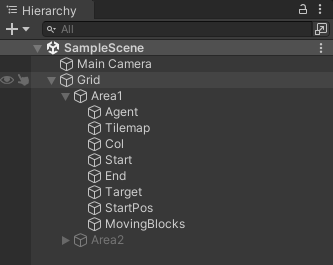
\includegraphics[width=12cm]{peliobjektilistaus.png}
\caption{Lista peliobjekteista avoimessa näkymässä. Sisäkkäiset peliobjektit ovat lapsiobjekteja.}
\label{peliobjektikuva}
\end{figure}

\subsection{Komponentit}

Komponentit antavat peliobjekteille ominaisuuksia ja toiminnallisuuksia kuten muodon, värin tai fysiikan \parencite{unitydoccomp}. Komponentteja voi olla rajattomasti, mutta peliobjektilla on luonnin jälkeen vähintään Transform-komponentti, joka määrittää peliobjektin sijainnin, suunnan ja skaalan. Transform-komponenttia ei voi poistaa peliobjektilta. Esimerkiksi valmis kolmiulotteinen objekti pallo saa automaattisesti Mesh Filter-, Mesh Renderer- ja Sphere Collider -komponentit. Kaksi ensimmäistä Mesh-komponenttia antavat pallolle graafiset ominaisuudet ja Sphere Collider fyysiset törmäysominaisuudet. Sphere Collider -komponentti asettuu automaattisesti pallon graafisen ulkomuodon kokoiseksi.

Usein komponenteilla on erilaisia arvoja, kuten koko tai väri, joita voi muokata käyttöliittymäelementtien avulla. Komponentit voivat sisältää myös viittauksia muihin peliobjekteihin, tiedostoihin tai assetteihin. Esimerkiksi Sprite Renderer -komponenttiin voidaan lisätä viittaus kuvatiedostoon, jolloin Unity renderöi peliobjektin kohdalle tai pinnalle lisätyn kuvan. Kuvassa \ref{komponenttikuva} on lista peliobjektin komponenteista ja niiden ominaisuuksista. Esimerkiksi kuvan Rigidbody 2D- ja Collider-komponentit antavat peliobjektille mahdollisuuden tunnistaa ja käsitellä törmäysdataa.

\begin{figure}[t]
\centering
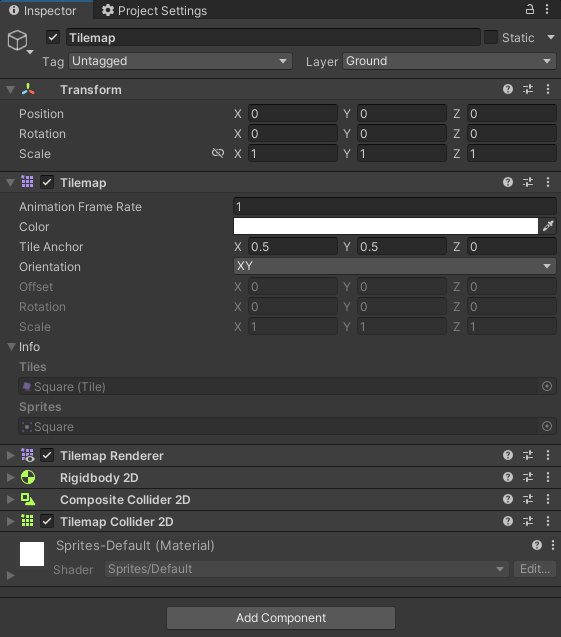
\includegraphics[width=12cm]{komponenttilistaus.png}
\caption{Lista peliobjektin komponenteista.}
\label{komponenttikuva}
\end{figure}

\subsection{Skriptit}

Ohjelmoinnin merkitys Unityn käytössä tulee skripteistä \parencite{unitydocscripts}. Skriptit ovat ohjelmakooditiedostoja, joita voi lisätä peliobjektiin komponenttien tavoin. Skripteissä voi esimerkiksi määritellä ominaisuuksia ja arvoja, joita voi muokata komponenttilistauksessa tai ajon aikana. Unity tukee tällä hetkellä vain C\#-ohjelmointikieltä, mutta tuki ennen myös Javascriptiin pohjautuvaa UnityScript-ohjelmointikieltä.

Unity tarjoaa skripteihin MonoBehaviour-pohjaluokan, joka mahdollistaa pelinkehityksen tärkeimmät osat eli Start()-aloitusfunktion ja Update()-päivitysfunktion. Start()-funktio ajetaan ennen yhtäkään päivitysfunktiota, joten siinä voidaan määrittää ja alustaa tarvittavat alkuarvot. Update()-funktio ajetaan joka ruudunpäivityskerralla, joten siihen sijoitetaan usein pelilogiikka ja mahdollisesti fyysiset toiminnallisuudet.

Skriptien avulla peliobjekteille voidaan tehdä lähes kaikki samat asiat kuin Unity Editorissa. Peliobjekteja voidaan etsiä tagien tai nimien kautta ja niille voidaan lisätä ja poistaa komponentteja ajon aikana. Käyttämättömät peliobjektit voidaan tuhota tai asettaa epäaktiivisiksi, jos niitä ei tarvita.

\section{Machine Learning Agents}

Machine Learning Agents on Unitylle kehitetty ilmainen koneoppimispaketti, joka mahdollistaa Unity Editorilla luotujen simulaatioympäristöjen ja Python APIn välisen vuorovaikutuksen \parencite{juliani2018unity}. ML-agents SDK (Software Development Kit) tarjoaa kaikki toiminnallisuudet ja skriptit toimivan koneoppimisympäristön luomiseen. Kuva \ref{mlagentsstructure} havainnollistaa yksinkertaisen ML-agents koneoppimisympäristön toimintaa.

\subsection{ML-agents SDK}

ML-agents SDK sisältää kolme ydinosaa: sensorit, agentit ja akatemia. Agentti-komponentti voidaan lisätä suoraan Unityn peliobjektille, jolloin se pystyy keräämään havaintoja ja suorittamaan toimintoja alueella ja vastaanottamaan palkkioita. Sensorit mahdollistavat havaintojen keräämisen eri tavoin. Akatemia ylläpitää tietoa simulaation askelmäärästä ja ympäristön parametreista sekä ohjaa agenttien toimintaa.

\begin{figure}[h]
\centering
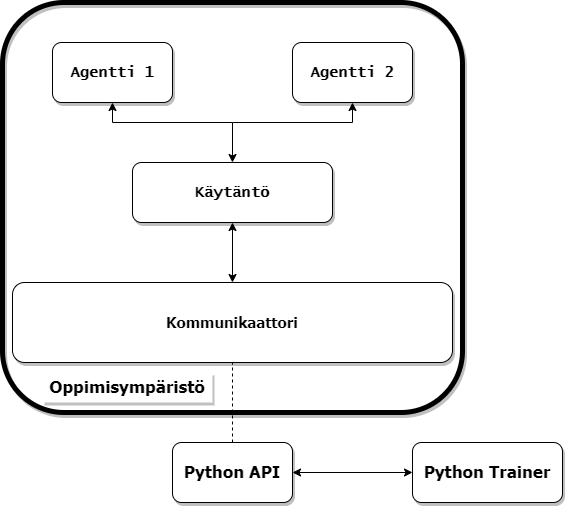
\includegraphics[width=10cm]{mlagents_structure.png}
\caption{Lohkokaavio Unity ML-agents-paketin toiminnasta.}
\label{mlagentsstructure}
\end{figure}

Agentin käytäntö määritellään Behavior Name -nimikkeen avulla. Eri agenteilla voi olla sama käytäntö, jolloin agentit käyttävät kyseistä käytäntöä päätöksentekoon. Myös useiden erilaisten agenttien toiminta voidaan mahdollistaa erinimisillä käytännöillä.

\subsection{Python API ja PyTorch}

Python APIa käytetään Unityllä tehdyn simulaatioympäristön ja koneoppimissilmukan käsittelyyn. APIn avulla tekijän ei tarvitse itse olla suoraan yhteydessä Pythonin koneoppimiskouluttajaan, vaan API tarjoaa helppokäyttöiset, valmiit menetelmät koneoppimissilmukan luomiseen. Tarkemmin APIsta ja sen toiminnasta voi lukea dokumentaatiosta\footnote{https://github.com/Unity-Technologies/ml-agents/blob/main/docs/Python-LLAPI-Documentation.md}.

PyTorch\footnote{https://pytorch.org/} on avoimen lähdekoodin koneoppimiskehys, johon pohjautuen Unity ML-agents-paketin koneoppimiseen liittyvät toteutukset on tehty. PyTorch sisältää kaikki syväoppimisen perusosat datan kanssa työskentelystä ja koneoppimismallin luomisesta mallin parametrien optimointiin ja oppimismallien tallentamiseen.

\chapter{Tutkimuksen empiirinen osuus}
\label{empiirinen}

Tässä luvussa käsitellään tutkimuksen empiiristä osuutta. Tutkimus toteutettiin empiirisenä vertailevana tutkimuksena. Vertailun kohteena olivat Unityn ML-agentin suorittama reitinhaku ja heuristiseen A*-algoritmiin perustuva reitinhaku. Luvussa \ref{sec:tutkimuksenkuvaus} kuvaillaan tutkimusta yleisellä tasolla ja esitellään tutkimuksessa käytetyt työkalut. Luvussa \ref{sec:tutkimusasetelma} käydään läpi simulaatioympäristöt ja koneoppimiseen liittyvät konfiguraatiot. Luvussa \ref{agenttihavainnot} kerrotaan koneoppimisagentin havainnoista ja palkkoista. Lopuksi luvussa \ref{sec:mittaaminen} käsitellään tulosten mittaamista.

\section{Tutkimuksen kuvaus}
\label{sec:tutkimuksenkuvaus}

Tässä luvussa kuvataan miten Unityä käytettiin tutkimuksessa ja millaisia alueita ja algoritmeja toteutettiin.

\subsection{Alueiden luonti}

Unityn valmiiden menetelmien avulla luotiin yksinkertaisia ruudukkoalueita, jonne sijoitettiin esteruutuja, kävelykelpoisia ruutuja ja alku- ja loppuruudut sekä joihinkin alueisiin liikkuvia esteitä. Ruudukon pohjana käytettiin Grid-komponenttia ja kävely- ja esteruutujen asetteluun Tilemap-komponenttia. Alueet ovat kooltaan 37x52 ruutua ja alueen ulkoreuna koostuu yhden ruudun paksuisesta esteestä.

\subsection{Unity}

Tutkimuksen simulaatioalustana käytettiin Unityä, koska sen käyttö oli ennestään tuttua ja se soveltuu hyvin erilaisten ympäristöjen ja tilanteiden simuloimiseen. Tutkimusta varten Unity Hubissa luotiin valmis 2D-projekti ja projektiin lisättiin Unity Package Managerin kautta ML-agents-paketti\footnote{https://docs.unity3d.com/Packages/com.unity.ml-agents@2.0/manual/index.html}, jotta tarvittavat toiminnallisuudet saatiin käyttöön koneoppimista varten. Unityllä luotiin agentti, joka on neljään mahdolliseen suuntaan liikkuva neliö. ML-agents-paketin avulla agentille annettiin viisi komponenttia. Behavior Parameters -komponentilla pystytään määrittelemään vektorihavaintojen lukumäärä ja tieto siitä, käyttääkö agentti valmista koneoppimismallia vai onko opettaminen käynnissä. Agent Script -komponentissa määritellään mitä vektorihavaintoja ylipäätään kerätään, mitä palkkioita agentti saa ja esimerkiksi mitä opetusjakson alussa tapahtuu. Decision Requester -komponentilla määritellään kuinka tasaisin väliajoin agentti tekee päätöksiä. Kaksi Ray Perception Sensor 2D -komponenttia mahdollistaa havaintojen keräämisen myös säteiden osumatiedoista. Agentin opettamiseen käytetään syvään vahvistusoppimiseen perustuvaa SAC-algoritmia.

\subsection{A*-algoritmi}

Reitinhaun vertailua varten toteutettiin A*-algoritmi. Agentti pystyy liikkumaan neljään suuntaan, joten A*-algoritmin heuristiikaksi valittiin Manhattan-etäisyys. A*-algoritmin toteutusta täytyi hieman muokata tutkimukseen sopivaksi. Pelialueet voivat muuttua reaaliaikaisesti, jolloin perinteinen A*-algoritmi ei pysty reagoimaan muutoksiin välittömästi. Algoritmia muokattiin tutkimukseen siten, että esteen ilmestyessä laskelmoidulle reitille A*-algoritmi ajetaan uudestaan, mutta lähtöpisteeksi asetetaan agentin uusi sijainti. Uusi sijainti on agentin siihen asti kulkema matka, jolloin seuraava reitinhakuiteraatio vaatii lyhyemmän matkan ja on kevyempi muistinkäytön kannalta. Ratkaisu ei kuitenkaan ole järkevä suuremmissa pelialueissa, mutta soveltuu hyvin tämän tutkimuksen esimerkkeihin.

\section{Tutkimusasetelma}
\label{sec:tutkimusasetelma}

Tässä luvussa kerrotaan millaisessa ympäristössä empiirinen osuus toteutettiin ja miten ympäristö konfiguroitiin tutkimuksen eri osioita varten.

\subsection{Alue}
\label{alue}

Tutkimuksessa toteutettiin kolme eri tason aluetta: helppo, keskivaikea ja vaikea. Helppo alue oli tehty tarkoituksella avaraksi ja alueella oli vain muutamia esteitä. Keskivaikeassa alueessa oli useampia esteitä ja seiniä ja alueelle pyrittiin tekemään sekä kapeita käytäviä että erillisiä huoneita. Kuvassa \ref{areabeginnerintermediate} nähdään helppo ja keskivaikea pelialue rinnakkain. Vaikea alue on sama kuin keskivaikea, mutta sinne tehtiin 1x1 suuruinen liikkuva este ja erillinen kolme ruutua pitkä portti, joka aukeaa ja sulkeutuu kahden sekunnin välein. Liikkuva este etenee yhden sekunnin välein kuvan \ref{areadifficult} punaisella merkityllä alueella ja toinen merkitty alue kuvaa portin sijaintia ja kokoa. Keskivaikean alueen koneoppimismallia käytettiin vaikean alueen testaamiseen, jotta voidaan testata agentin sopeutumista dynaamisiin esteisiin. Koneoppimista varten kohderuutu valittiin Unityn valmiilla Random.Range()-funktiolla satunnaisesti vapaiden ruutujen seasta, mutta vaikean alueen testauksessa ruutuja valittiin esteiden läheisyydestä tai niiden toiselta puolelta. Vertailussa kohteet valittiin käsin tasaisesti alueen reunoilta.

\begin{figure}[h]
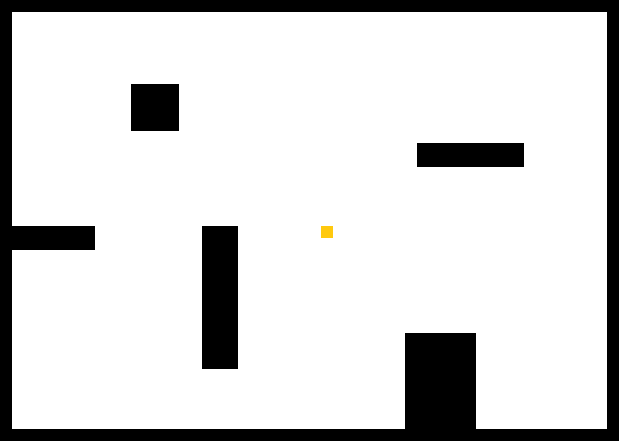
\includegraphics[width=7cm]{area_beginner.png}
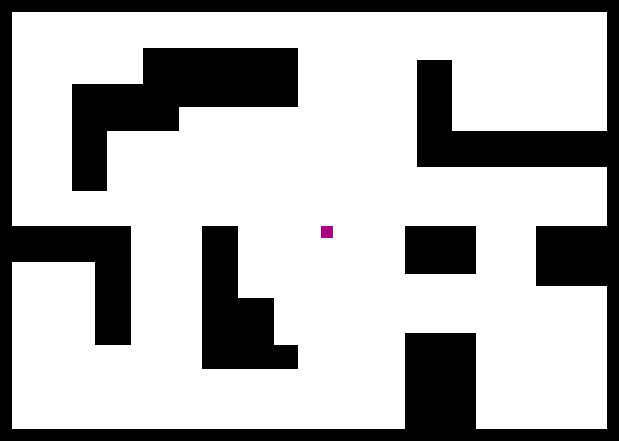
\includegraphics[width=7cm]{area_intermediate.png}
\centering
\caption{Helppo ja keskivaikea pelialue. Keltainen ruutu pelialueen keskellä on agentti.}
\label{areabeginnerintermediate}
\end{figure}

\begin{figure}[h]
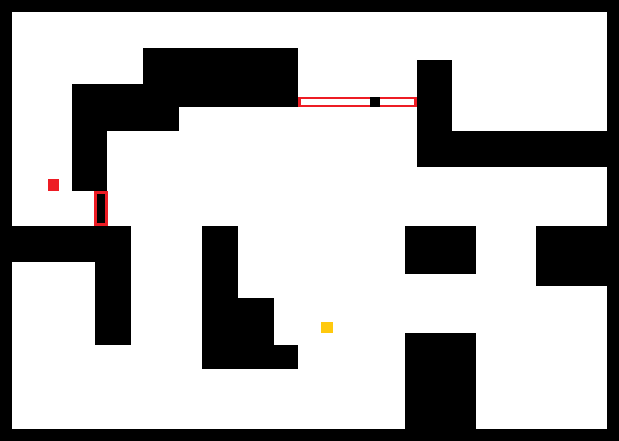
\includegraphics[width=13cm]{area_difficult.png}
\centering
\caption{Vaikea pelialue, jossa on merkitty punaisilla ääriviivoilla tasaisin väliajoin aukeava portti ja liikkuva este. Keltainen ruutu on agentti ja punainen ruutu on kohderuutu.}
\label{areadifficult}
\end{figure}

\subsection{Koneoppiminen}
\label{koneoppiminenasetelma}

Agentilla voi olla käytössä sekä \textit{Continuous Actions}- että \textit{Discrete Actions} -taulukoita, jotka syötetään parametrina OnActionReceived()-funktioon. Continuous Actions -taulukon voivat olla mitä arvoja tahansa, mutta ne rajataan ennalta [-1,...,1] välille. Kyseiset arvot voidaan asettaa esimerkiksi agentin liikkumista varten, jolloin agentti pystyy oppimisen aikana kontrolloimaan arvoja. Toisena vaihtoehtona on Discrete Actions -taulukko, joka sisältää vain kokonaislukuja. Tässä tutkimuksessa agentilla on käytössä vain viiden elementin Discrete Actions -taulukko, jossa on arvot [0,1,2,3,4]. Agentin liikkuminen on toteutettu siten, että 0 on paikallaan pysyminen, 1 on liikkuminen vasemmalle, 2 on liikkuminen oikealle, 3 on liikkuminen alas ja 4 on liikkuminen ylös. Agentti pystyy liikkumaan kerralla yhden ruudun verran.

Unity ML-agents mahdollistaa saman pelialueen rinnakkaisen opettamisen yksinkertaisella drag-and-drop-menetelmällä. Pelialueesta luodaan prefab eli valmis malli, joita voidaan siirtää useampi kappale samalle näkymälle. Kaikki agentit pystyvät keräämään kokemuksia samaan käytäntöön, kunhan jokaisella on sama Behavior Name -arvo. Opettaminen aloitetaan virtuaaliympäristössä komennolla \texttt{mlagents-learn <polku kon\-fi\-gu\-raa\-ti\-o\-tie\-dos\-toon> --run-id=<opetustunnus>}. Opettaminen käynnistetään Unity Editorissa Play-painikkeella. Yksi opetusjakso kestää 1000 askeletta tai kunnes agentti saapuu maaliin tai osuu esteeseen.

Agentin opettamisessa käytettiin samoja hyperparametreja eli konfiguraatiotiedostoa kuin Unityn valmiissa koneoppimisesimerkissä nimeltä Food Collector\footnote{https://github.com/Unity-Technologies/ml-agents/blob/main/docs/Learning-Environment-Examples.md\#food-collector}. Food Collector -pelissä koneoppimisagentti pyrki keräämään pelialueelta vain tiettyjä ruokia ja oppi väistelemään kiellettyjä ruokia. Pelin idea oli hyvin lähellä tämän tutkimuksen esimerkkiä, joten tässä tutkimuksessa päädyttiin samoihin hyperparametreihin. Ainoastaan \textit{max\_steps} asetettiin miljoonaan, jolloin oppiminen pysäytettiin automaattisesti siihen. Myös \textit{summary\_freq}-arvoksi vaihdettiin 10000, jolloin opetusta pystyttiin seuraamaan tiheämmin aikavälein. Kokonaisuudessaan konfiguraatio-tiedoston sisältö löytyy liitteenä tutkimuksen lopusta luvusta \ref{liitteet} ja hyperparametrien kuvaukset Unity ML-agents GitHubista \footnote{https://github.com/Unity-Technologies/ml-agents/blob/main/docs/Training-Configuration-File.md}.

Opettamista voidaan seurata komentoriviltä, joka näyttää 10000 askeleen välein kuluneen ajan sekunneissa ja palkkioiden keskiarvon ja keskihajonnan. Tämän lisäksi tarkempaa kehittymistä voi seurata Tensorboardin\footnote{https://github.com/Unity-Technologies/ml-agents/blob/main/docs/Using-Tensorboard.md} avulla komennolla \texttt{tensorboard --logdir re\-sults --port 6006} ja menemällä selaimella sivulle localhost:6006. Tässä tutkimuksessa seurattiin agentin kumulatiivista palkkiota (engl. cumulative reward), entropian määrää mallissa eli kuinka satunnaisia agentin toiminnot ovat, kustannusfunktion häviön keskiarvoa (engl. policy loss) ja arvofunktion häviön keskiarvoa (engl. value loss). Näiden neljän mittarin perusteella voidaan arvioida agentin käytännön kehittymistä opetuksen aikana. Tässä tutkimuksessa kuvaajia ei tasoitettu ollenkaan.

Helpon tason alueessa opettamista tehtiin 500000 askeleen ajan, joka kesti 2712 sekuntia. Keskivaikean tason alueessa opetettiin miljoonan askeleen ajan, joka kesti 5600 sekuntia. Molemmista alueista muodostui .onnx-päätteinen malli-tiedosto, jonka pystyy asettamaan agentille käyttöön Behavior Parameters -komponentissa. Keskivaikean tason luomaa neuroverkkoa sovellettiin vaikean tason alueen reitinhakuun, jotta pystyttiin tarkastella agentin sopeutumista uusiin esteisiin.

\section{Agentin havainnot ja palkkiot}
\label{agenttihavainnot}

Koneoppimisagentin oppimista ohjaavat sen tekemät havainnot ja sen saamat palkkiot. Havaintoja voi tallentaa suoraan skriptitiedostossa käsin AddObservation()-metodilla, jolle annetaan parametrina datatyyppi ja sen arvo. Tämän tutkimuksen reitinhakutehtävissä agentti havainnoi omaa ja kohteen sijaintia kaksiulotteisessa vektorimuodossa \((x,y)\), jolloin jokaisella askeleella neuroverkko saa tiedon näistä sijainneista. Tähän havaintoon käytetään Unityn omaa datatyyppiä Vector2, joka sisältää \(x\) ja \(y\) arvot float-tyyppisinä. Lisäksi agentti havainnoi sen etäisyyttä kohteeseen, jonka laskemiseen käytetään Unityn valmista Vector2.Distance() -funktiota. Agentille lisättiin myös kaksi Ray Perception Sensor 2D -kom\-po\-nent\-ti\-a, jotka lähettävät agentista osumatietoja kerääviä säteitä. Ensimmäinen sensori sisältää kaksitoista sädettä, jotka ovat pituudeltaan 15 yksikköä ja tunnistavat ainoastaan kohderuudun. Toinen sensori sisältää kahdeksan sädettä etäisyydeltään viisi yksikköä ja tunnistavat vain esteruutuja. Tunnistaminen määritellään erillisen Detectable Tags -kentän avulla, johon kirjoitetaan tunnistettavan kohteen tagi. Esteet ovat tagilla Col ja kohderuutu tagilla End. Lisäksi sensorille annetaan Ray Layer Mask -valintalistaan tieto, mihin alueen kerroksiin säteet voivat fyysisesti osua ja mitkä kerrokset jätetään huomiotta. Tässä tutkimuksessa esteet on asetettu kerrokselle Collision ja kohderuutu kerrokselle End. Näiden tietojen perusteella sensori lähettää automaattisesti säteiden osumadatan float-taulukkona neuroverkolle, jolloin sitä ei tarvitse itse toteuttaa Agent Script -tiedostossa.

Agentin saamat palkkiot ovat vahvistusoppimisen ydin ja tässä tapauksessa agenttia palkitaan sen nopeuden ja yleisen suoriutumisen perusteella. Jokaisen agentin päätöksen yhteydessä annetaan pieni negatiivinen palkkio, jolloin agenttia ohjataan suorittamaan tehtävä niin nopeasti kuin mahdollista. Palkkio määritellään skriptitiedostossa AddReward(-1/\textit{MaxStep}), jossa \textit{MaxStep} on yhden opetusjakson maksimipituus eli kuinka monta päätöstä agentti voi yhden jakson aikana tehdä. Tässä tutkimuksessa pelialueet ovat melko pieniä, joten maksimipituudeksi asetettiin 1000. Jos agentti ei saa suoritettua tehtävää ja maksimi askelmäärä saavutetaan, agentti saa palkkioksi yhteensä -1. Jos agentti osuu kohteeseen, sille annetaan koko jakson palkkioksi +1 eli SetReward(1). Jos agentti yrittää liikkua matkalla esteruutuun, sille annetaan palkkioksi -1 eli AddReward(-1) ja opetusjakso pysäytetään. Tällä halutaan estää agentin turha törmääminen esteisiin.

\section{Tulosten mittaaminen}
\label{sec:mittaaminen}

A*-algoritmin reitin selvittämistä ja koneoppimisagentin toimintaa on vaikea mitata ajallisesti, koska agentti ei laske reittiä ennalta toisin kuin A*-algoritmi. Tässä tutkimuksessa vertaillaan siksi sekä kohteeseen liikkumiseen kulunutta aikaa että käytyjä solmuja ja esitellään saatu data taulukkomuodossa. Sekä koneoppimiseagentti että A*-algoritmia käyttävä agentti pystyvät liikkumaan yhden ruudun joka 0.2 sekunti. Ajan mittaamista varten toteutettiin ajastin, joka alkoi nollasta pelin käynnistyttyä. Kun koneoppimisagentti tai A*-algoritmia käyttävä agentti saapui kohteeseen, ajastimen sen hetkinen aika ja agentin käytyjen solmujen lukumäärä tulostettiin Unityn sisäiseen debuggauslokiin ja kirjattiin sieltä talteen. Jos agentti ei päässyt kohteeseen tuhannen päätösaskeleen kuluessa, tehtävä lopetettiin ennenaikaisesti ja agentin ajaksi ja solmujen lukumääräksi asetettiin epäonnistui. Tämän lisäksi tarkastellaan laadullisesti molempien vaihtoehtojen reittien optimaalisuutta eli esimerkiksi tekeekö koneoppimisagentti turhia liikkeitä verrattuna A*-algoritmin optimaaliseen reittiin. Dynaamisissa alueissa tutkitaan koneoppimisagentin tekemiä ratkaisuja A*-algoritmin ratkaisuihin ja selitetään sanallisesti niiden eroja.

Koneoppimisagentin opettamisen kehitystä seurataan Tensorboardin avulla. Tensorboardin kuvaajista kumulatiivinen palkkio kertoo agentin jaksojen palkkioiden keskiarvon, jonka tulisi kasvaa oppimisen yhteydessä. Entropia-kuvaaja esittää agentin toimintojen satunnaisuutta. Aluksi entropian kuuluisi olla suurta, mutta agentin oppiessa entropian tulisi tasaisesti laskea. SAC-algoritmin luonteeseen kuuluu entropian maksimointi, joten entropian kuuluisi hieman vaihdella agentin selvitellessä uusia tiloja. Käytännön virhefunktio kuvaa agentin käytännön muuttumista ja sen tulisi laskea onnistuneen oppimisen aikana. Arvofunktio kuvaa mallin kykyä ennustaa tilojen arvoja. Sen tulisi aluksi kasvaa oppimisen aikana ja lopuksi laskea kun palkkio tasoittuu.

\chapter{Tulokset ja johtopäätökset}
\label{tulokset}

Tässä luvussa esitellään tutkimuksen tulokset. Luvussa \ref{helppo} esitetään helpon pelialueen koneoppimisen tuloksia. Luvussa \ref{keskivaikea} esitetään keskivaikean pelialueen koneoppimisen tulokset. Luvussa \ref{vaikea} kerrotaan keskivaikean neuroverkkomallin sopeutumisesta vaikean pelialueen dynaamisuuteen. Luvussa \ref{vertailu} esitellään A*-algoritmin ja koneoppimisagentin vertailun tulokset. Lopuksi luvussa \ref{johtop} kerrotaan johtopäätökset tuloksista ja mahdolliset rajoitteet tutkimuksessa.

\section{Helppo pelialue}
\label{helppo}

Koneoppimisagentin opettaminen aloitettiin helposta pelialueesta. Kuvasta \ref{beginnercumulativeentropy} huomataan, että agentin kumulatiivinen keskiarvopalkkio nousi tasaisesti ylöspäin kohti maksimia eli yhtä, kunnes noin 220000 askeleen jälkeen kehitystä ei suuremmin tapahtunut. Aluksi agentti testasi satunnaisesti toimintoja ja sensoridatasta saatuja havaintoja huomatakseen eri toimintojen ja palkkioiden merkityksen. Seiniin osuminen aiheuttaa tässä tapauksessa ison menetyksen palkkiossa, joten agentti oppi nopeasti välttelemään osumia. Satunnaiset kontaktit maaliruutujen kanssa saivat agentin huomaamaan sijainti- ja sensoridatan yhteyden positiivisen palkkion saamiseen, joten agentti alkoi pyrkimään kohti lähimpiä maaliruutuja. Alueen kauimmaiset maaliruudut eivät kuitenkaan olleet helppoja tapauksia, joten niiden oppimiseen meni useita kymmeniä tuhansia opetusaskeleita. Lopulta agentti oppi kiertämään esteet ja saavutti jopa reunimmaiset maaliruudut vaivattomasti. Opettamista ei kuitenkaan kannattanut jatkaa liian pitkään, jotta liialliselta ylisovittamiselta vältyttäisiin. Opettaminen lopetettiin siksi ennenaikaisesti 500000 askeleen kohdalla.

Kuvasta \ref{beginnercumulativeentropy} näkee myös, että agentin entropian määrä laski aluksi nopeasti. Onnistuneen oppimisen aikana entropian tulisi laskea samalla, kun palkkioiden määrä kasvaa. Helpon alueen tapauksessa tämä toteutui, joka viestii onnistuneesta oppimisesta. Kuvasta \ref{beginnerloss} nähdään agentin käytännön virhefunktion ja arvofunktion keskiarvohäviö. Käytännön virhefunktio laskee nopeasti 150000 askeleen kohdalla, kun agentti saa käsityksen oikeasta toiminnasta. Arvofunktion kuvaajassa esiintyy piikkimäisiä nousuja ja laskuja, mutta pitkällä aikavälillä sekin laskee tasaisesti. Kokonaisuudessaan agentti oppi maksimoimaan palkkion määrän ja onnistui suurimmaksi osin ratkaisemaan annetut reitinhakuongelmat.

\begin{figure}[h]
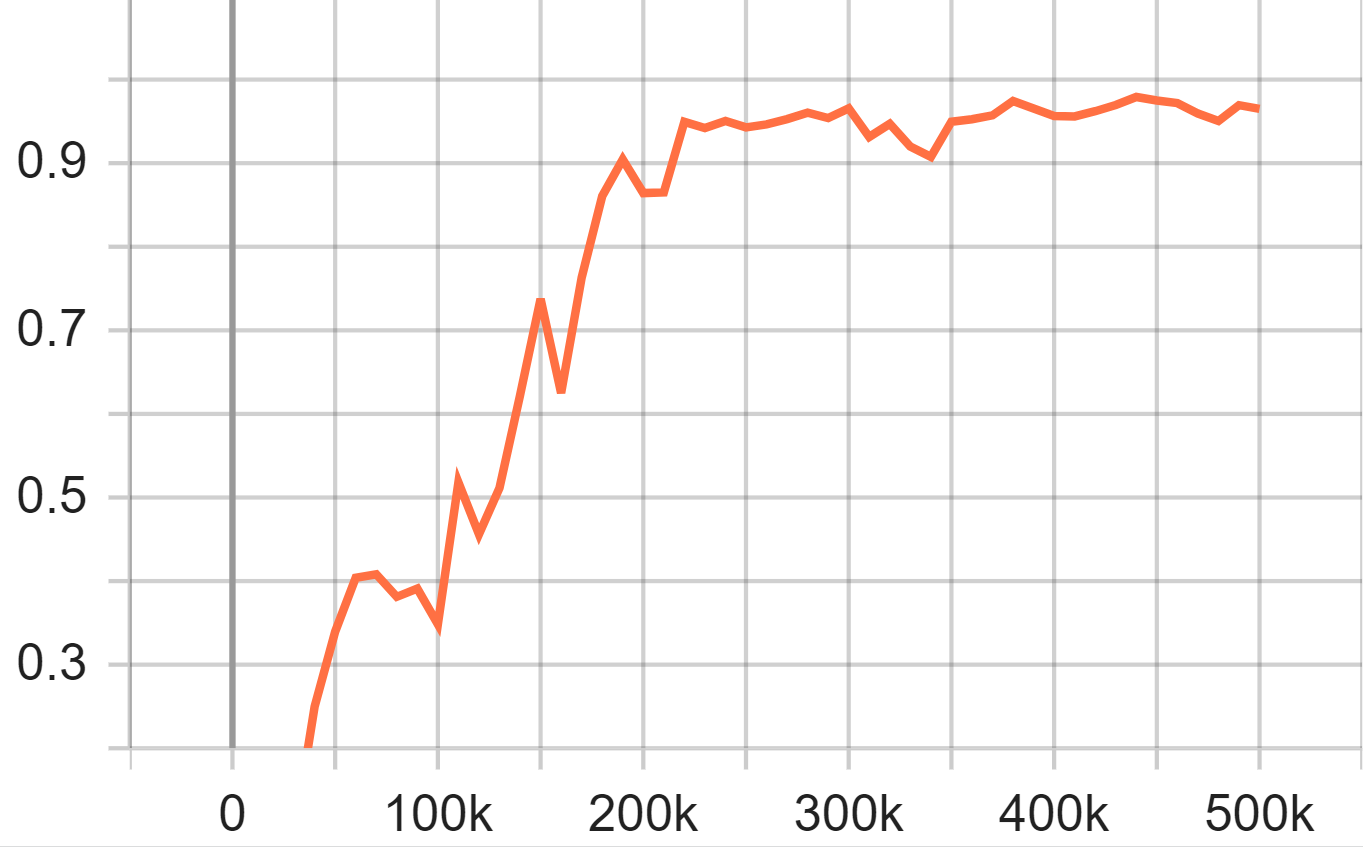
\includegraphics[width=7cm]{B_Cumulative_Reward.png}
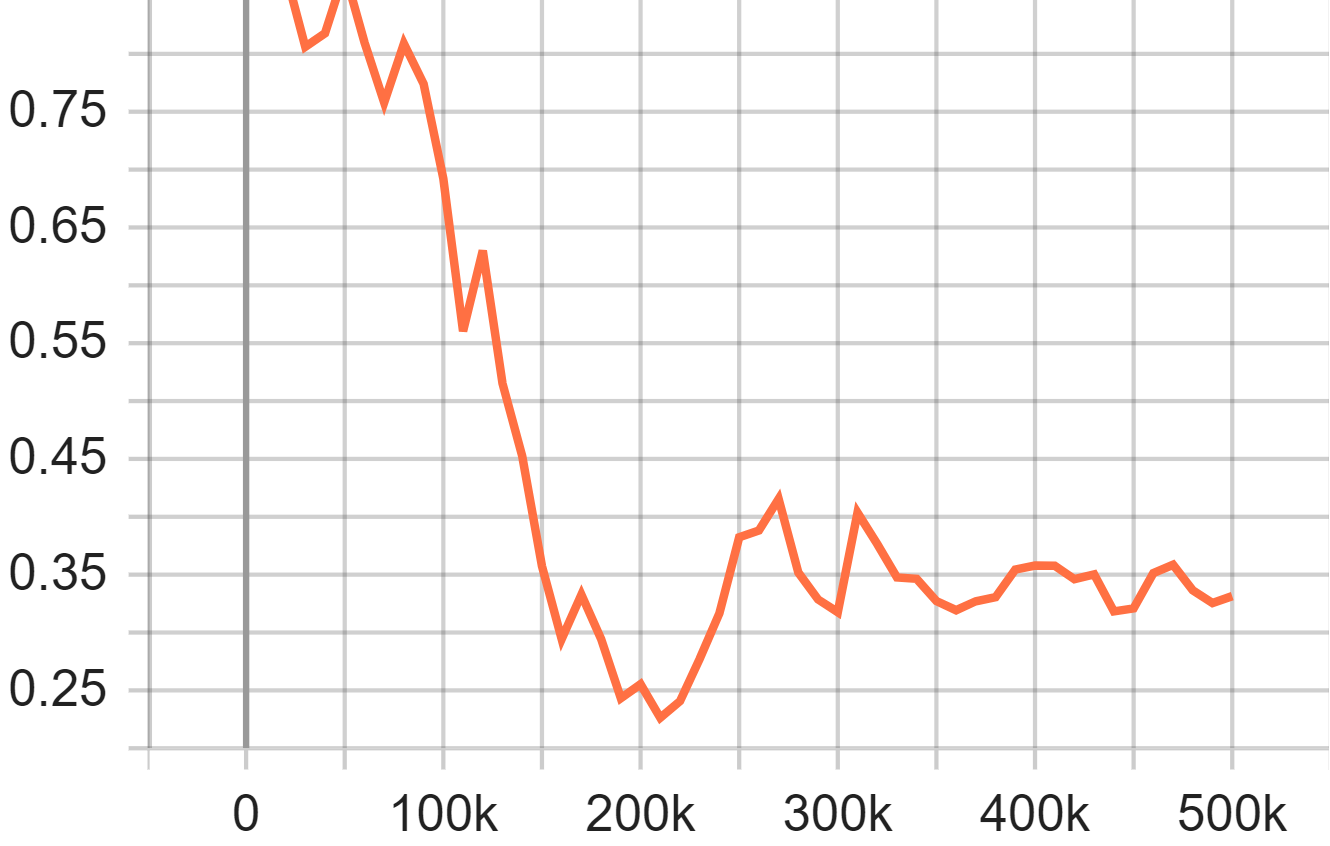
\includegraphics[width=7cm]{B_Policy_Entropy.png}
\caption{Vasemmalla helpon tason kumulatiivinen palkkio ja oikealla entropian kehitys 500000 askeleen aikana.}
\label{beginnercumulativeentropy}
\end{figure}

\begin{figure}[h]
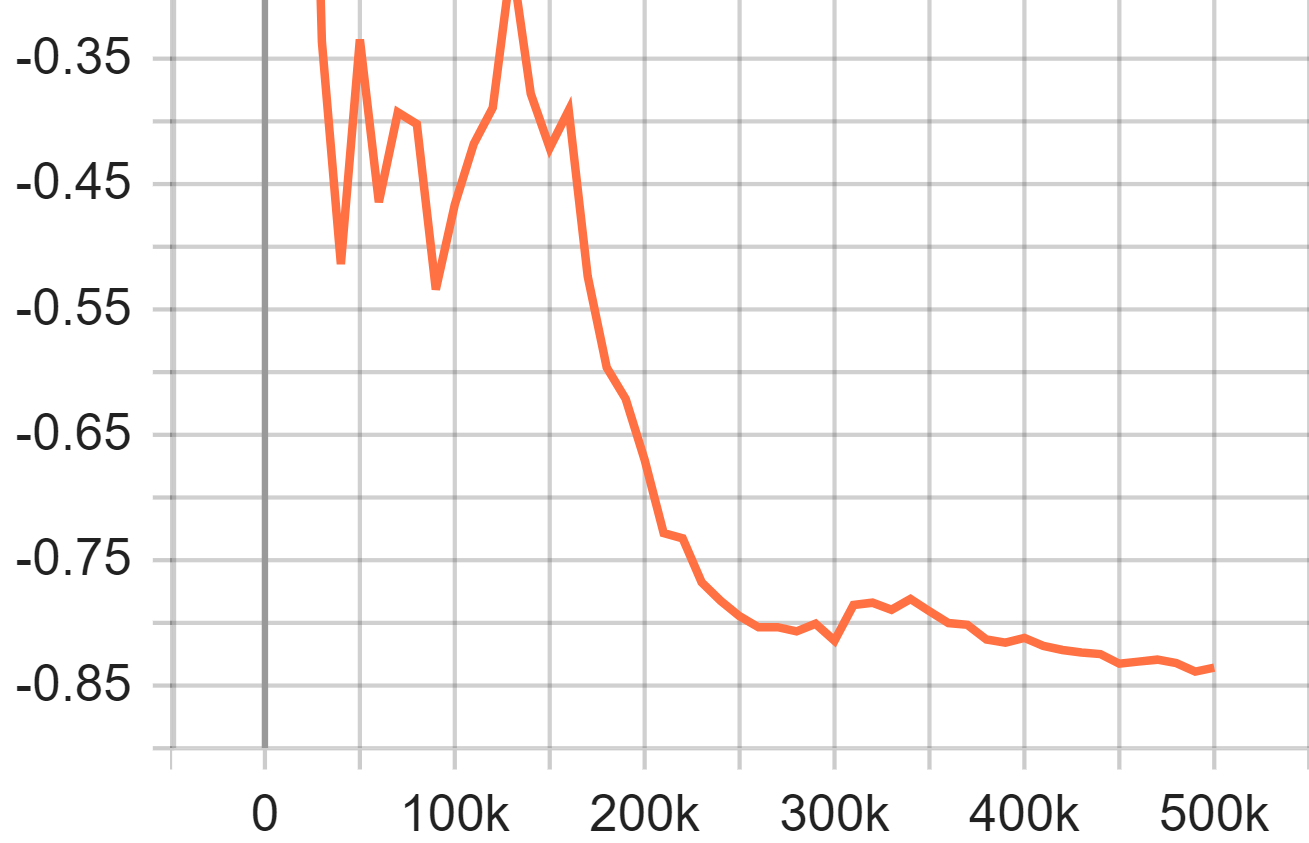
\includegraphics[width=7cm]{B_Policy_Loss.png}
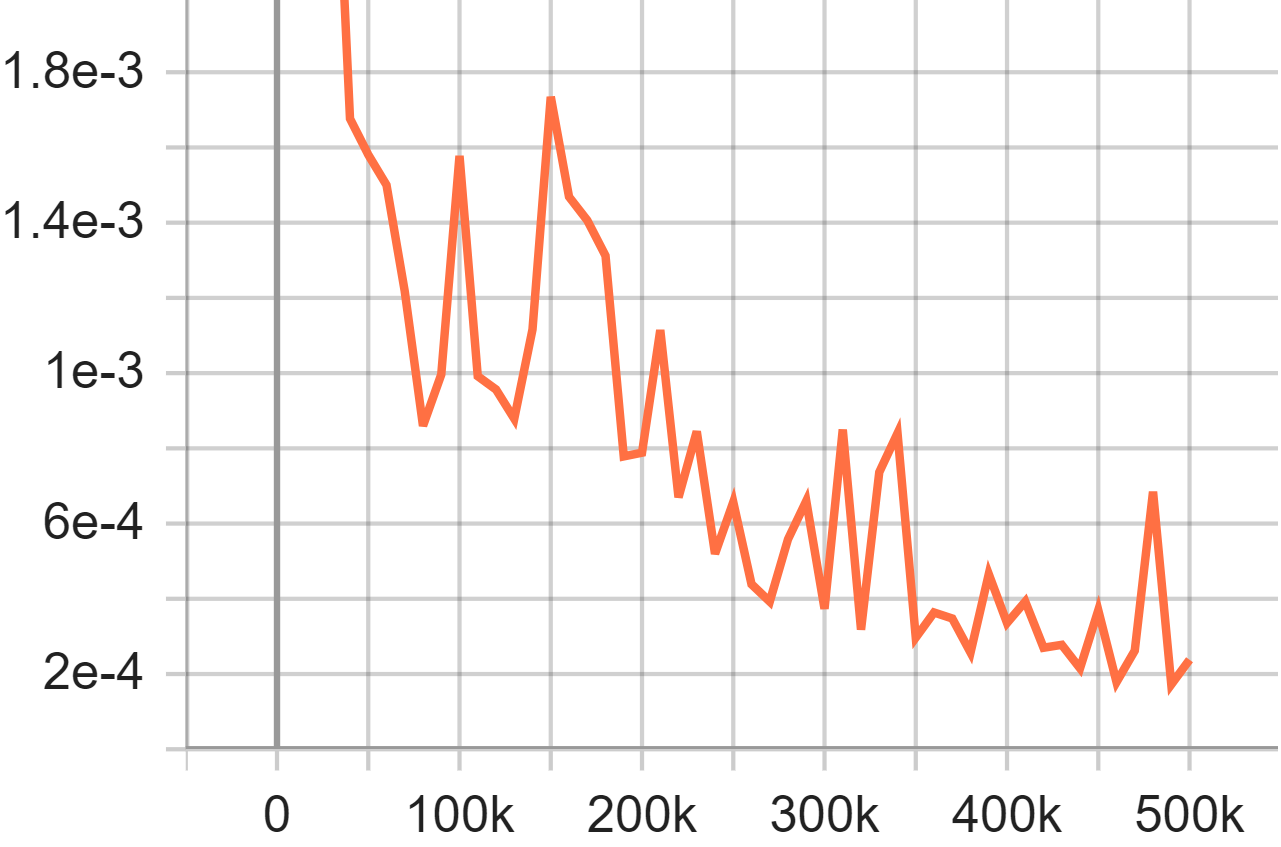
\includegraphics[width=7cm]{B_Value_Loss.png}
\caption{Vasemmalla helpon tason käytännön virhefunktion kehitys ja oikealla arvofunktion kehitys 500000 askeleen aikana.}
\label{beginnerloss}
\end{figure}

\section{Keskivaikea pelialue}
\label{keskivaikea}

Keskivaikeassa alueessa koneoppimisagentti kehittyi selvästi hitaammin, joka näkyy myös kuvasta \ref{intermediatecumulativeentropy}. Vasta 200000 askeleen kohdalla agentti alkoi saamaan keskiarvoltaan positiivista palkkiota. Oppiminen oli kuitenkin tehokasta 600000 askeleeseen asti, jonka jälkeen se hidastui merkittävästi saavuttaessaan noin arvon 0.9. Keskivaikean alueen lisääntyneet esteet tekivät alun oppimisesta hidasta, koska agentti pyrki aluksi maksimoimaan palkkion määrän pysymällä kaukana esteistä. Agentti liikkui pitkään vain aloitusruudun ympärillä, mutta entropian kasvaessa se onnistui liikkumaan myös pidemmälle alkuruudusta. Entropian kuvaajasta huomaa, että entropian määrä laski nopeasti 200000 askeleeseen asti, jonka jälkeen se vaihteli loppuajan 0.3 ja 0.5 välillä.

Kuvan \ref{intermediateloss} virhefunktion keskiarvo kasvaa jostain syystä alussa 300000 askeleeseen asti, jonka jälkeen se laskee hitaasti. Alussa oppimisessa on selvästi ollut hankalaa ja agentti ei välttämättä ole pystynyt oppimaan tehokkaasti, kuten palkkion kehityksestä myös huomattiin. Arvofunktio sen sijaan laskee alussa jyrkästi ja nousee sen jälkeen hieman 200000 ja 400000 askeleen välillä ja lopuksi laskee hitaasti ja tasoittuu opetuksen loppuun mennessä.

\begin{figure}[h]
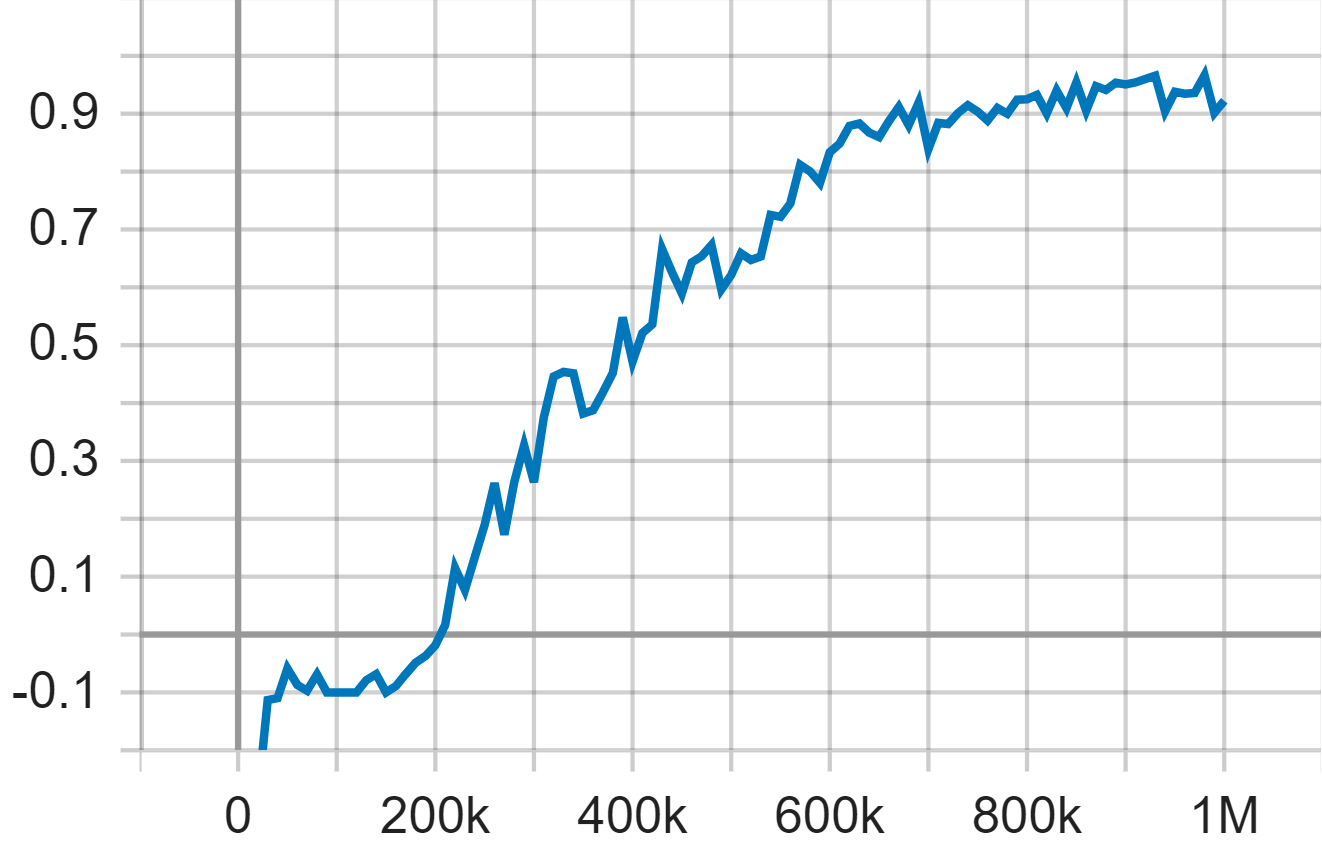
\includegraphics[width=7cm]{I_Cumulative_Reward.png}
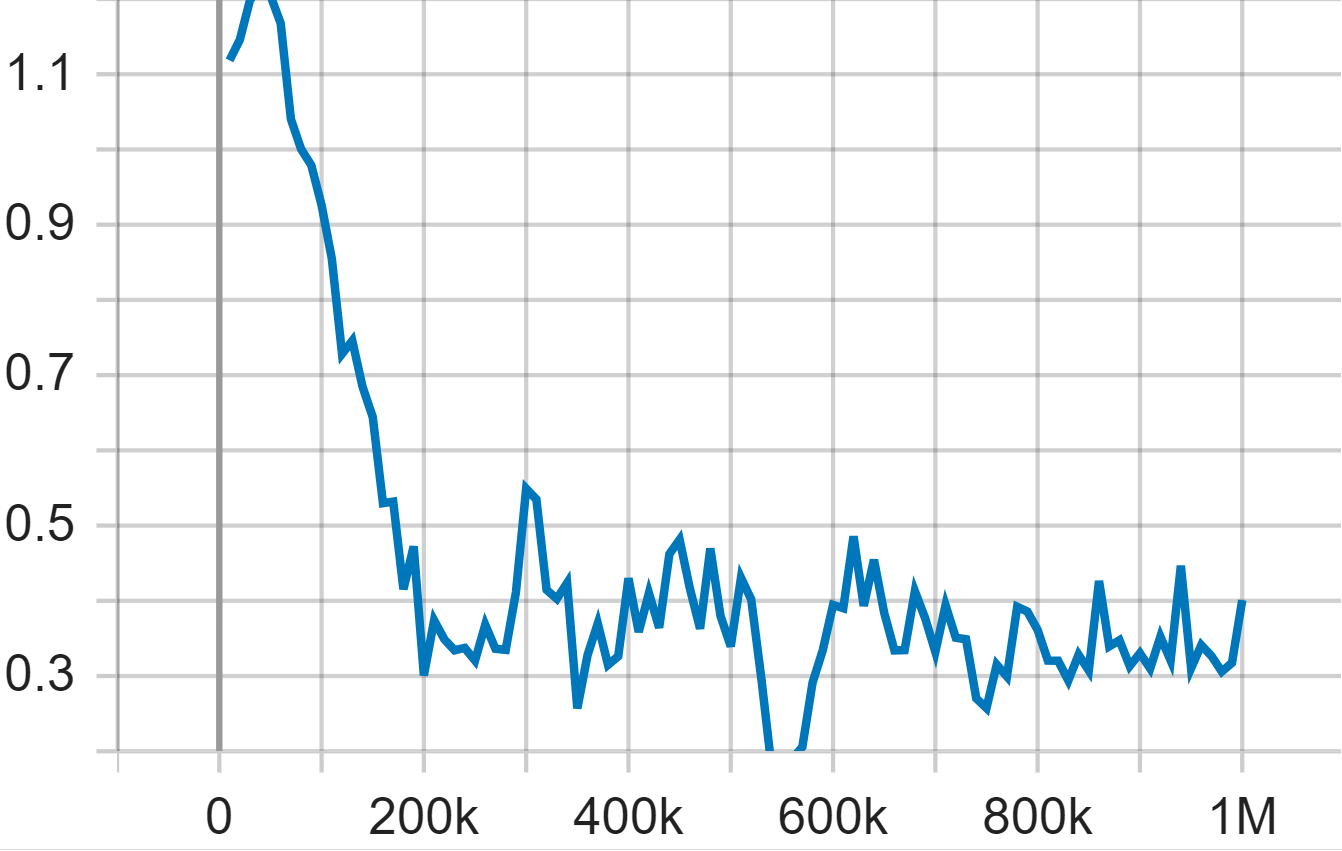
\includegraphics[width=7cm]{I_Policy_Entropy.png}
\caption{Vasemmalla keskivaikean tason kumulatiivinen palkkio ja oikealla entropian kehitys miljoonan askeleen aikana.}
\label{intermediatecumulativeentropy}
\end{figure}

\begin{figure}[h]
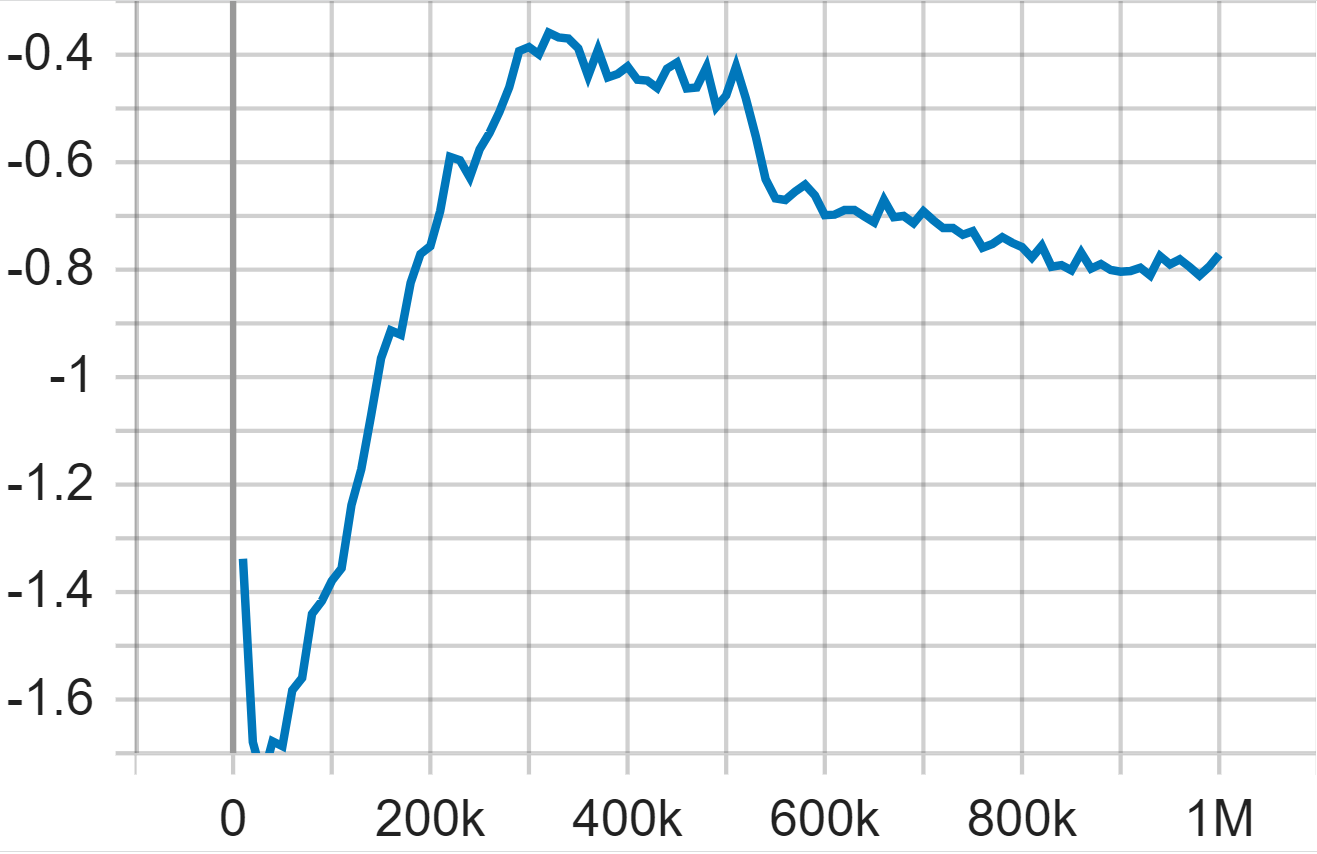
\includegraphics[width=7cm]{I_Policy_Loss.png}
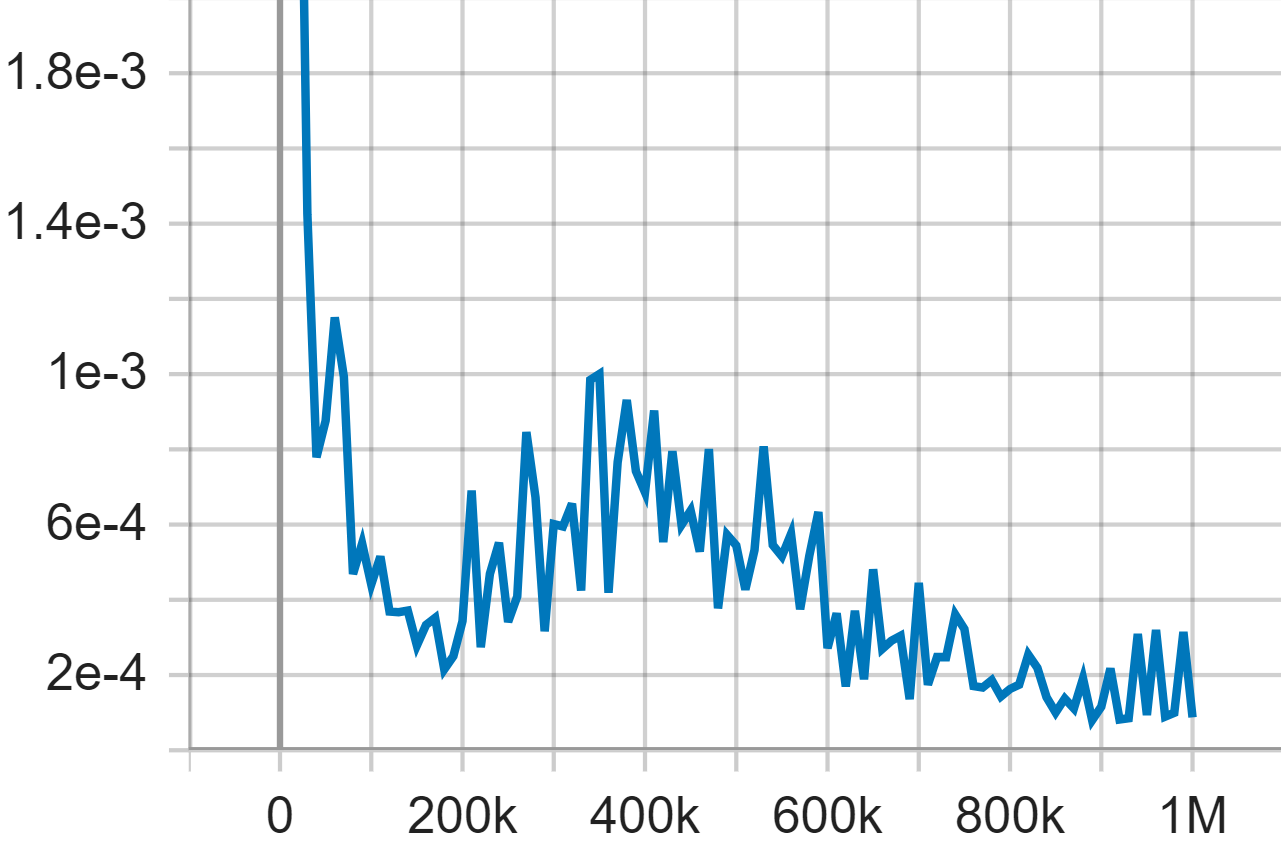
\includegraphics[width=7cm]{I_Value_Loss.png}
\caption{Vasemmalla keskivaikean tason käytännön virhefunktion kehitys ja oikealla arvofunktion kehitys miljoonan askeleen aikana.}
\label{intermediateloss}
\end{figure}

\section{Vaikea pelialue}
\label{vaikea}

Keskivaikean tason opetuksen luomaa .onnx-tiedostoa käytettiin vaikean tason reitinhakuongelmiin, jolloin pystytään arvioimaan agentin sopeutumista dynaamisen alueen reitinhakuun. Agentti kohtasi reitillään uusia yllättäviä esteitä, joita ei opetusprosessissa esiintynyt. Reitinhakua testattiin aluksi portin toiselle puolelle. Agentti liikkui oppimansa mukaan kohti aukinaista porttia, mutta portin sulkeutuessa agentti pysähtyi muutaman ruudun päähän odottamaan. Kun portti avautui uudestaan, agentti eteni kohderuutuun normaalisti. Kuvasta \ref{agentgate} nähdään agentin päätöksentekoa portin ollessa auki ja kiinni. Kuvasta myös huomataan, että agentti liikkui turhaan pystysuunnassa ennen porttia, joka kertoo epäoptimaalisesta reitistä. Optimaalisin vaihtoehto olisi siirtyä heti portin viereen odottamaan. Seuraavaksi testattiin agentin sopeutumista liikkuvaan esteeseen. Agentti varoi estettä monen ruudun päästä, joka johtui todennäköisesti liian pitkistä sensorisäteistä. Monissa tapauksissa agentti ei uskaltanut lähteä kiertämään estettä, vaan jäi liikkumaan esteen väärälle puolelle sivusuunnassa. Joissain tapauksissa agentti väisti esteen ja eteni kohderuuduun.

\begin{figure}[h]
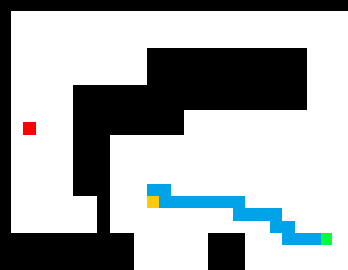
\includegraphics[width=7cm]{agent_avoid_gate.png}
\hspace{1 cm}
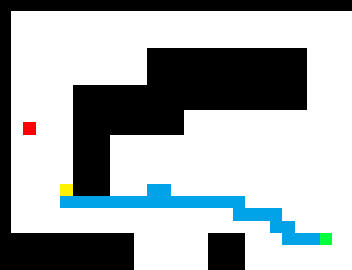
\includegraphics[width=7cm]{agent_through_gate.png}
\caption{Agentti osasi odottaa portin avautumista ja käytti portin läpi kulkevaa reittiä kohteeseen. Punainen ruutu on kohde, vihreä ruutu on aloitusruutu ja keltainen ruutu on agentti. Siniset ruudut kuvaavat agentin kulkemaa reittiä.}
\label{agentgate}
\end{figure}

\section{A*-algoritmin ja koneoppimisagentin vertailu}
\label{vertailu}

A*-algoritmi suoriutuu staattisista pelialueista optimaalisesti, joten helpon ja keskivaikean pelialueen vertailua ei toteutettu. Taulukossa \ref{vertailutaulukko} nähdään kymmenen eri reitinhakutilanteen tulokset vaikeassa pelialueessa, jossa on liikkuvia esteitä. Kohteiden sijainnit nähdään kuvassa \ref{testtargets}. Unityn fysiikkapäivitykset tapahtuvat arvon \textit{Time.fixedDeltaTime} perusteella, joka on oletuksena 0.02 sekuntia. Tämän vuoksi taulukossa nähdään joissain tilanteissa sama määrä käytyjä solmuja, mutta ajat eroavat noin 0.02 sekuntia toisistaan.

\begin{table}[htp]
\centering
\caption{Agentin ja A*-algoritmin vertailutaulukko.}
\label{vertailutaulukko}
\begin{tabular}{cccccc}
\hline
Kohde & Agentin aika (s) & A* aika (s) & Agentin solmut (n) & A* solmut (n) & Ero (\%) \\
\hline \hline
1 & 6.8196 & 16.6600$^*$ & 35 & 84$^*$ & 140 \\

2 & 8.6198 & 7.0392 & 44 & 36 & -18 \\

3 & 4.0196 & 3.2396 & 21 & 17 & -19 \\

4 & Epäonnistui & 6.8397 & Epäonnistui & 35 & -- \\

5 & 4.4196 & 4.4399 & 23 & 23 & 0 \\

6 & 6.6195 & 6.6396 & 34 & 34 & 0 \\

7 & 3.6197 & 3.6399 & 19 & 19 & 0 \\

8 & 4.8198 & 3.8399 & 25 & 20 & -20 \\

9 & Epäonnistui & 3.8398 & Epäonnistui & 20 & -- \\

10 & 9.8198 & 7.6598 & 50 & 39 & -22 \\

\hline

\end{tabular}

$^*$A* kohtasi portin ja valitsi pidemmän reitin sen seurauksena.

\end{table}

\begin{figure}[h]
\centering
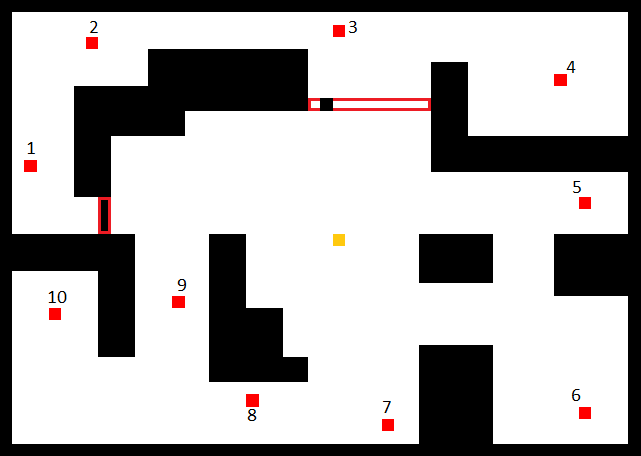
\includegraphics[width=12cm]{area_difficult_test_targets.png}
\caption{A*-algoritmin ja koneoppimisagentin vertailun kohderuudut.}
\label{testtargets}
\end{figure}

Taulukosta kohteista viisi, kuusi ja seitsemän huomataan, että koneoppimisagentti onnistuu suoraviivaisissa ja lähialueen reitinhaussa optimaalisesti ja samassa ajassa kuin A*-algoritmi. Ensimmäisessä kohteessa hyödynnettiin portin olemassaoloa. Agentti onnistui odottamaan portin aukeamista, kuten luvussa \ref{vaikea} selitettiin. Kuva \ref{astargate} havainnollistaa A*-algoritmin toimintaa kohdatessaan portin. A*-algoritmi päätyi valitsemaan aluksi portin läpi kulkevan reitin, mutta kohdatessaan sulkeutuneen portin se vaihtoi kokonaan reittiään. Kiertoreitin kulkeminen vei tässä tapauksessa selvästi pidemmän ajan, jolloin koneoppimisagentti päätyi suorittamaan reitinhakutehtävän nopeammin.

\begin{figure}[h]
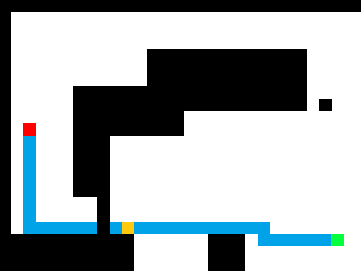
\includegraphics[width=7cm]{a_star_gate_collision.png}
\hspace{1 cm}
\vspace{1 cm}
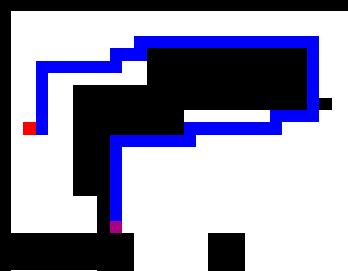
\includegraphics[width=7cm]{a_star_detour.png}
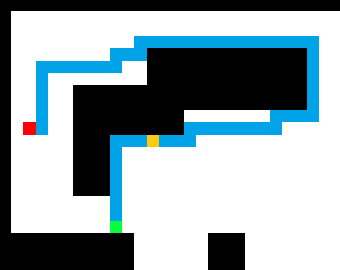
\includegraphics[width=7cm]{a_star_detour_no_gate.png}
\caption{A*-algoritmin valitsema reitti portin ollessa auki ja kiinni. Punainen ruutu on kohde, vihreä ruutu on aloitusruutu ja keltainen ruutu on agentti. Siniset ruudut kuvaavat A*-algoritmin laskemaa reittiä.}
\label{astargate}
\end{figure}

Toinen kohde aiheutti hieman ongelmia agentin reitinhaussa ja se päätyi valitsemaan epäoptimaalisen reitin portin läpi, kun taas A*-algoritmi valitsi optimaalisen reitin liikkuvan esteen vierestä. Kolmannen kohteen tehtävässä agentti varoi liikkuvaa estettä jo melko kaukaa, jolloin reitinhaku ei ollut optimaalista. A*-algoritmi ehti mennä esteen ohi. Neljännen kohteen reitinhaussa agentti epäonnistui eikä koskaan saavuttanut kohdetta. Kahdeksannessa kohteessa agentti jostain syystä valitsi pysyä aluksi paikallaan, joka laskettiin myös mukaan solmujen lukumäärään. Yhdeksäs kohde epäonnistui jälleen agentilta, joka oli yllätys, koska kohde oli hyvin lähellä vain yhden esteen takana. Kymmenes kohde sen sijaan onnistui, mutta jälleen epäoptimaalisesti hitaampaa reittiä pitkin. Yleisesti käytyjen solmujen erot eivät olleet suuria. Koneoppimisagentti oli useimmiten vain 20\% hitaampi kuin A*-algoritmi kohteissa, joissa eroa havaittiin. Parhaimmillaan koneoppimisagentti oli yli kaksi kertaa nopeampi opitun käyttäytymisen ansiosta.

Liikkuvan esteen suhteen A*-algoritmi toimi selvästi paremmin kuin koneoppimisagentti. Tutkimuksessa toteutettu A* variaatio onnistui heti vaihtamaan reittiä kohdatessaan esteen, jolloin se pääsi kiertämään sen välittömästi. Ääritapauksissa A* valitsi kiertoreitin samalta puolelta johon este oli liikkumassa, jolloin este liikkui heti uudestaan reitille ja A* joutui laskemaan reitin jälleen uudestaan. Agentti sen sijaan oli liian varovainen liikkuvan esteen suhteen, kuten luvussa \ref{vaikea} selitettiin. Pahimmillaan agentti ei pystynyt suorittamaan reitinhakutehtävää ollenkaan.

\section{Johtopäätökset ja rajoitteet}
\label{johtop}

A*-algoritmi suoriutuu selvästi staattisista pelialueista optimaalisesti. Dynaamisissa alueissa sen suoriutuminen riippuu vahvasti esteiden toteutuksesta. A*-algoritmi osaa väistellä liikkuvia, yksittäisiä esteitä laskemalla uuden reitin välittömästi uudestaan. Lisäksi uusi reitti on suurella todennäköisyydellä lyhyempi ja siten käyttää vähemmän muistia. Suuremmat esteet, jotka estävät pääsyn kokonaan tietyn reitin kautta hetkellisesti, osoittautuivat vaikeiksi, koska A*-algoritmi ryhtyi kiertämään kohteeseen toista kautta. Uusi reitti voi olla pahimmillaan monta kertaa pidempi. Tässäkin tapauksessa esteen luonne tosin vaikuttaa A*-algoritmin reitin optimaalisuuteen. Jos este tulisi reitille pysyvästi, niin A*-algoritmin toiminta olisi hyväksyttävää. Jos reitti estyy vain hetkellisesti, niin A*-algoritmin uuden reitin valinta olisi huono päätös. A*-algoritmia kannattaa käyttää edelleen videopelien reitinhakuun ja etenkin uusien variaatioiden käyttöä kannattaa myös harkita.

Koneoppimisagentin reitinhaku oli yksinkertaisissa alueissa lähes moitteetonta. Oppiminen oli helpossa pelialueessa suoraviivaista ja nopeaa, mutta keskivaikea alue oli aluksi ongelmallinen ja agentti ei saanut käsitystä oikeanlaisesta käytännöstä. Jotkin reunatapaukset aiheuttivat agentille ongelmia sekä helpossa että keskivaikeassa alueessa, jolloin se päätyikin liikkumaan vain paikallaan eikä löytänyt kohteen luokse ajoissa. Agentti pystyi jollain tapaa sopeutumaan vaikean pelialueen esteisiin, vaikka se ei opetellut erikseen esteiden väistämistä. Koneoppimista voi suositella käytettävän alueissa, joihin liittyy jonkinlaista älyä kuten hetkellisesti estyviä reittejä.

A*-algoritmin toteutus oli hyvin yksinkertainen, jonka takia se ei täysin sovellu vertailukohteeksi. Tutkimuksessa olisi ollut parempi käyttää esimerkiksi D*- tai D* Lite -algoritmin tapaista dynaamisen alueen algoritmia, mutta niiden toteutus on selvästi hankalampaa eikä selkeitä ohjeita välttämättä löydy. Myös tässä tutkimuksessa toteutettu jatkuva A*-algoritmin uudelleenlaskenta esteiden tullessa reitille on tehotonta \parencite{stentz1995focussed}. Tämän tutkimuksen pelialueet ovat kuitenkin pieniä, joten A*-algoritmin tehokkuudella ei tässä tapauksessa ole merkitystä. Jos tutkimusta laajennettaisiin ja pelialueita tehtäisiin lisää, niin A*-algoritmi kannattaisi toteuttaa myös uudestaan tehokkaammin.

Koneoppimisagentin toteuttamisen suhteen on myös mahdollista toimia toisin. Vektorihavainnot ovat näihin yksinkertaisiin tapauksiin sopivat, mutta sensorihavaintoja voisi käyttää toisin. Säteet oli tässä tutkimuksessa jaettu kahteen osaan tunnistamaan erikseen esteitä ja kohdetta. Kohdesäteet olivat pitkiä ja menivät esteiden läpi ja estesäteet olivat lyhyempiä ja pysähtyivät esteisiin. Agentti oppi liiankin hyvin varomaan esteitä, jolloin liikkuvat esteet pysäyttivät sen etenemisen kokonaan. Estesäteet olisivat voineet olla lyhyempiä kuten esimerkiksi vain yhden ruudun pituisia. Agentti olisi voinut myös käyttää visuaalisia havaintoja, jotka olisivat syöttäneet suoraan agentin lähialueen pikselidataa neuroverkolle. Visuaaliset havainnot voisivat parantaa agentin käyttäytymistä esteiden läheisyydessä. Palkkiot oli toteutettu siten, että agenttia ohjattiin suorittamaan tehtävä mahdollisimman nopeasti lisäämällä jokaiselle aika-askeleelle negatiivista palkkiota. Ongelmaksi kuitenkin muodostui positiivisen palkkion harvinaisuus, koska agentti osui aluksi harvoin kohteeseen. Toteutukseen olisi voitu lisätä pieni palkkio, joka riippuisi agentin etäisyydestä kohteeseen ja testata vaikutusta kohteen löytämiseen. Yksi suurimmista muutoksista olisi hyperparametrien oikeanlainen konfigurointi, koska tässä tutkimuksessa oli käytössä valmiin esimerkin hyperparametrit. Suuremmat \textit{batch\_size} ja \textit{buffer\_size} arvot vaikuttaisivat gradientin ja kokemuspuskurin (engl. experience buffer) suuruuteen, jolloin agentti oppisi enemmän aiemmista kokemuksista. Myös esimerkiksi piilokerrosten (\textit{num\_layers}) lisääminen kahteen voisi tehostaa agentin toimintaa ongelmien kasvaessa suuriksi.

\chapter{Yhteenveto}
\label{yhteenveto}

Tässä tutkimuksessa pyrittiin pääasiassa selvittämään, voiko koneoppimista hyödyntää videopelien reitinhaussa ja miten reitinhaku vertautuu perinteisen A*-algoritmin ratkaisuihin. Vastausta haettiin seuraaviin tutkimuskysymyksiin

\begin{enumerate}
\item Oppiiko koneoppimisagentti suorittamaan reitinhakutehtäviä?
\item Miten koneoppimisagentin suorittama reitinhaku vertautuu A*-algoritmiin nopeuden ja tarkkuuden osalta?
\item Löytyykö reitinhakutehtävä, jota A*-algoritmi ei pysty ratkaisemaan, mutta koneoppimisagentti pystyy?
\end{enumerate}

Ensimmäiseen kysymykseen vastattiin empiirisessä osuudessa luomalla koneoppimisympäristö Unity-pelinkehitysalustalla käyttäen ML-agents-pakettia. Koneoppimisagentti käytti syvää vahvistusoppimista ja Soft Actor-Critic -algoritmia oppiakseen reitinhakutehtäviä hyväksikäyttämällä saatuja havaintoja ja palkkioita. Oppimisen kehitystä seurattiin Tensorboard-työkalun avulla ja saadut tulokset esiteltiin sanallisesti kuvaajia apuna käyttäen.

Toiseen kysymykseen vastattiin tutkimuksen empiirisessä osiossa vertailun muodossa. Koneoppimisagentti opetettiin keskivaikeassa alueessa ja koneoppimismallia käytettiin vaikean eli dynaamisen alueen reitinhakuun. Vaikeassa alueessa valittiin kymmenen kohdetta tasaisesti alueen reunoilta, jotka toimivat reitinhakutehtävien loppupisteinä. Tämän jälkeen verrattiin jokaiseen reitinhakutehtävään kulunutta aikaa ja käytyjä solmuja sekä koneoppimisagentin että A*-algoritmin osalta. Yhdessä reitinhakutehtävässä koneoppimisagentti onnistui suorittamaan reitinhakutehtävän nopeammin kuin A*-algoritmi, mutta yhdeksässä tehtävässä se suoriutui joko huonommin tai yhtä optimaalisesti kuin A*-algoritmi.

Kolmanteen kysymykseen vastattiin luomalla alueelle dynaamisia esteitä, jotka ovat tunnetusti A*-algoritmin heikkous. Neljässä reitinhakutehtävässä kymmenestä oli mukana dynaamisia esteitä, joista A*-algoritmi suoriutui kuitenkin melko hyvin. Tämän lisäksi A*-algoritmin ja koneoppimisagentin reitinhakua seurattiin esteiden läheisyydessä tarkemmin ja esitettiin tuloksia sanallisesti. Tässä tutkimuksessa ei kuitenkaan löydetty reitinhakutehtävää, jota A*-algoritmi ei olisi saanut suoritettua.

Tutkimus osoitti kuitenkin, että koneoppimisen avulla voidaan luoda reitinhakuagentteja, jotka pystyvät suorittamaan erilaisia reitinhakutehtäviä videopeleissä. Etenkin syvä vahvistusoppiminen soveltuu tehtävään lähes täydellisesti. Vastaavaa tutkimusta on esiintynyt lähinnä robotiikassa, joka kuitenkin sisältää omat rajoitteensa esimerkiksi turvallisuuden ja tehon suhteen. Videopeleissä rajoitteita ei ole niin paljon, joten agentin opettamisesta saadaan tehokkaampaa. Koneoppimisessa ei välttämättä kannata keskittyä pelkästään reitinhakuun, vaan agentti voidaan samalla opettaa ratkaisemaan muita pelillisiä tai loogisia ongelmia. Opettaminen voi kestää kauemmin, mutta agenteista saadaan siten yleishyödyllisiä.

\printbibliography

\chapter{Liitteet}
\label{liitteet}

\begin{verbatim}
behaviors:
  GraduTest:
    trainer_type: sac
    hyperparameters:
      learning_rate: 0.0003
      learning_rate_schedule: constant
      batch_size: 256
      buffer_size: 2048
      buffer_init_steps: 0
      tau: 0.005
      steps_per_update: 10.0
      save_replay_buffer: false
      init_entcoef: 0.05
      reward_signal_steps_per_update: 10.0
    network_settings:
      normalize: false
      hidden_units: 256
      num_layers: 1
      vis_encode_type: simple
    reward_signals:
      extrinsic:
        gamma: 0.99
        strength: 1.0
    keep_checkpoints: 5
    max_steps: 1000000
    time_horizon: 64
    summary_freq: 10000
    threaded: false
\end{verbatim}

\end{document}
